\documentclass[11pt]{article}
\usepackage[margin=0.75in]{geometry}
\usepackage{graphicx}
\usepackage{float}
\usepackage{booktabs}
\usepackage{multirow}
\usepackage{array}
\usepackage{fancyhdr}
\usepackage{titlesec}
\usepackage{amsmath}
\usepackage{amsfonts}
\usepackage{url}
\usepackage{hyperref}
\usepackage{xcolor}
\usepackage{caption}
\usepackage{subcaption}

% Page setup
\pagestyle{fancy}
\fancyhf{}
\rfoot{\thepage}
\renewcommand{\headrulewidth}{0pt}

% Section formatting
\titleformat{\section}{\large\bfseries}{\thesection}{1em}{}
\titleformat{\subsection}{\normalsize\bfseries}{\thesubsection}{1em}{}

% Custom colors
\definecolor{darkblue}{RGB}{0,0,139}
\definecolor{darkred}{RGB}{139,0,0}

% Improve text justification
\usepackage{microtype}
\setlength{\parindent}{0pt}
\setlength{\parskip}{6pt}
\usepackage{ragged2e}
\justifying

\begin{document}

% Cover Page
\begin{titlepage}
\centering
\vspace*{1.5cm}

% Main title with enhanced styling
{\Huge\bfseries\color{darkblue} The Beauty Inflection Point}\\[0.4cm]
{\LARGE\color{darkred} Emerging Market Investment Opportunities in Global Beauty}\\[0.8cm]

% Horizontal line for visual separation
\rule{0.8\textwidth}{2pt}\\[1cm]

% Subtitle section with better spacing
{\large\textbf{Strategic Analysis:} Income Thresholds and Market Acceleration}\\[0.5cm]
{\normalsize Cross-Country Statistical Evidence for Beauty Consumption Breakouts}\\[0.3cm]
{\normalsize with Focus on India's Investment Potential}\\[1.5cm]

\vspace{10cm}

% Author and date with enhanced formatting
{\Large\textbf{Arnav Jaitly}}\\[0.3cm]
{\normalsize August 2025}

\vfill

% Footer with professional touch
{\footnotesize Based on World Bank \& UN Comtrade Data | Statistical Analysis \& Modeling}

\end{titlepage}

\newpage

% Executive Summary
\section*{Executive Summary}
\addcontentsline{toc}{section}{Executive Summary}

This report analyzes beauty consumption across 11 countries to evaluate emerging market opportunities, focusing on India's potential. We conduct comprehensive statistical exploration to identify income-beauty relationships, comparative benchmarking against peer countries at similar development stages, and rigorous hypothesis testing across beauty categories to establish evidence-based investment insights.

\textbf{Key Findings:}
\vspace{-5pt}
\begin{itemize}
    \setlength{\itemsep}{-2pt}
    \item \textbf{India underperforms}: Trajectory significantly below successful emerging market peers (Figure 1a shows India's beauty share evolution vs benchmark countries)
    \item \textbf{Beauty as luxury}: Strong income-beauty correlation across all countries with 2.3x elasticity (Figure 1b demonstrates clear luxury good behavior)
    \item \textbf{Growth acceleration}: Beauty consumption increases faster than GDP growth over 30-year periods (Figure 2)
    \item \textbf{Strategic categories}: Skincare and women's beauty show strongest acceleration potential
    \item \textbf{Catalyst effects}: Countries can break through thresholds earlier than natural income progression
\end{itemize}

\vspace{-10pt}
\begin{figure}[H]
\centering
\begin{subfigure}[b]{0.48\textwidth}
    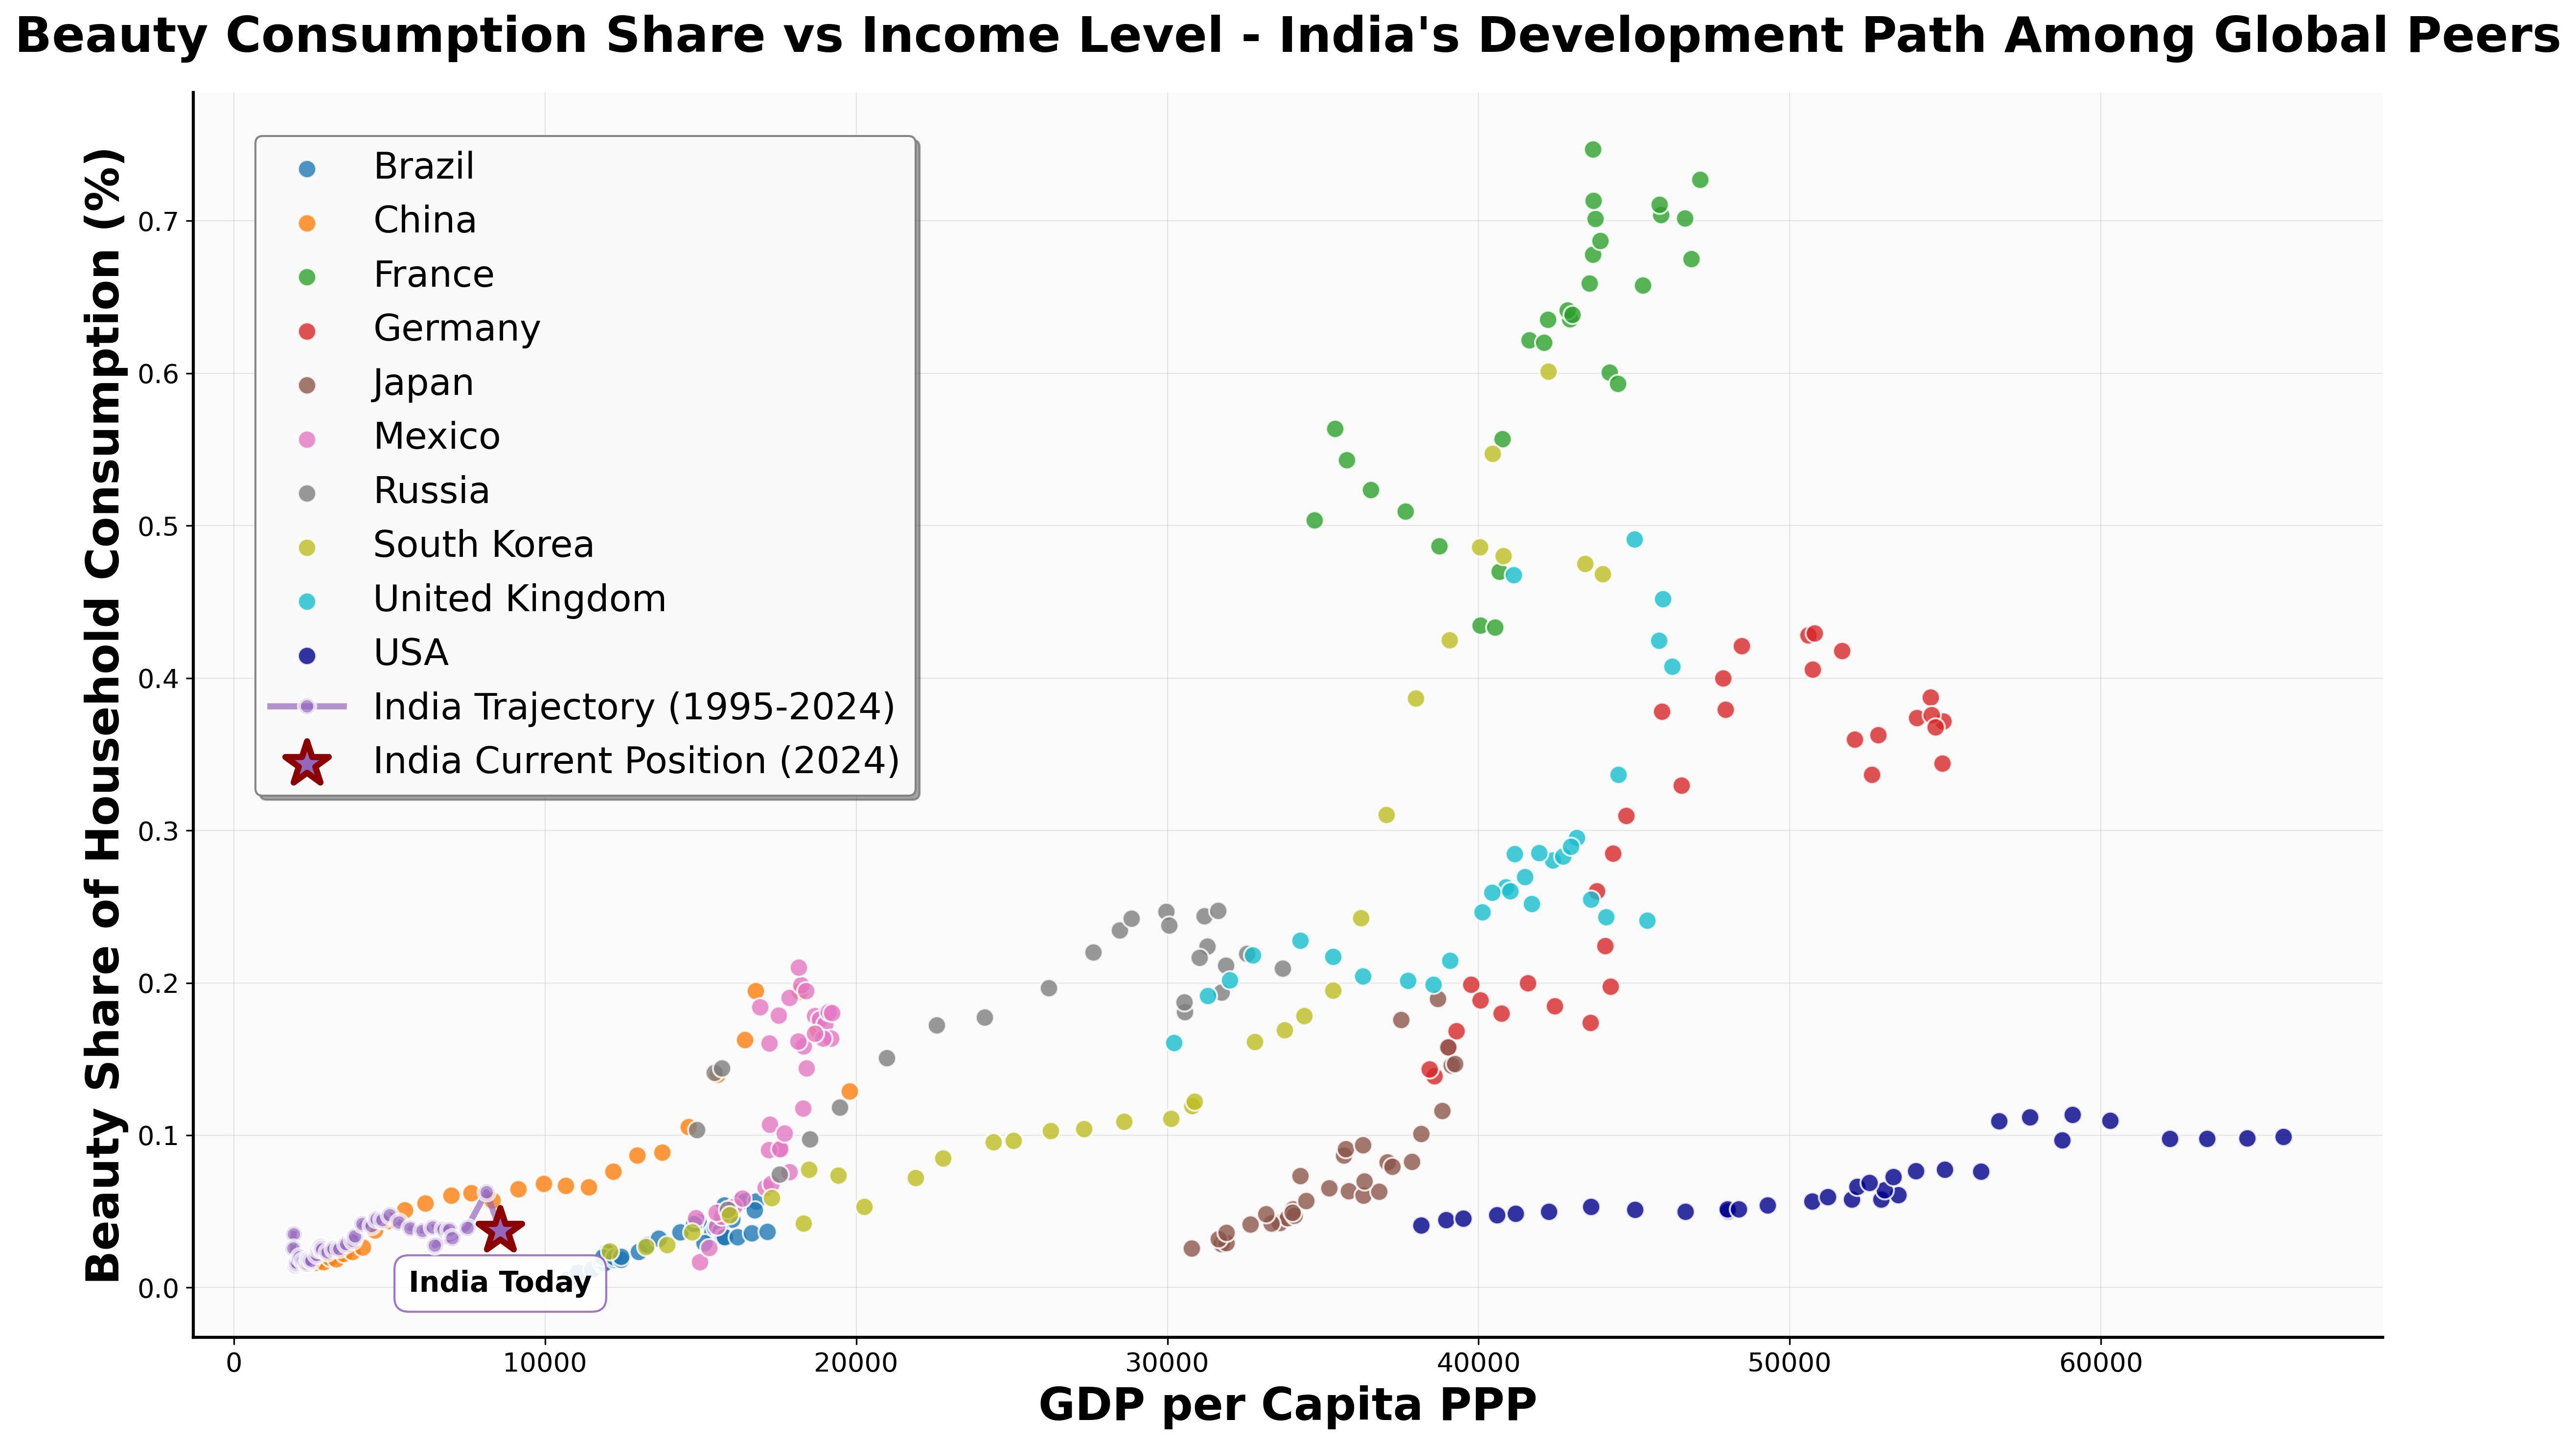
\includegraphics[width=\textwidth]{T2-3_beauty_share_overlay.png}
    \caption{\textbf{India's Growth Trajectory}: Significant gap vs successful emerging market patterns}
\end{subfigure}
\hfill
\begin{subfigure}[b]{0.48\textwidth}
    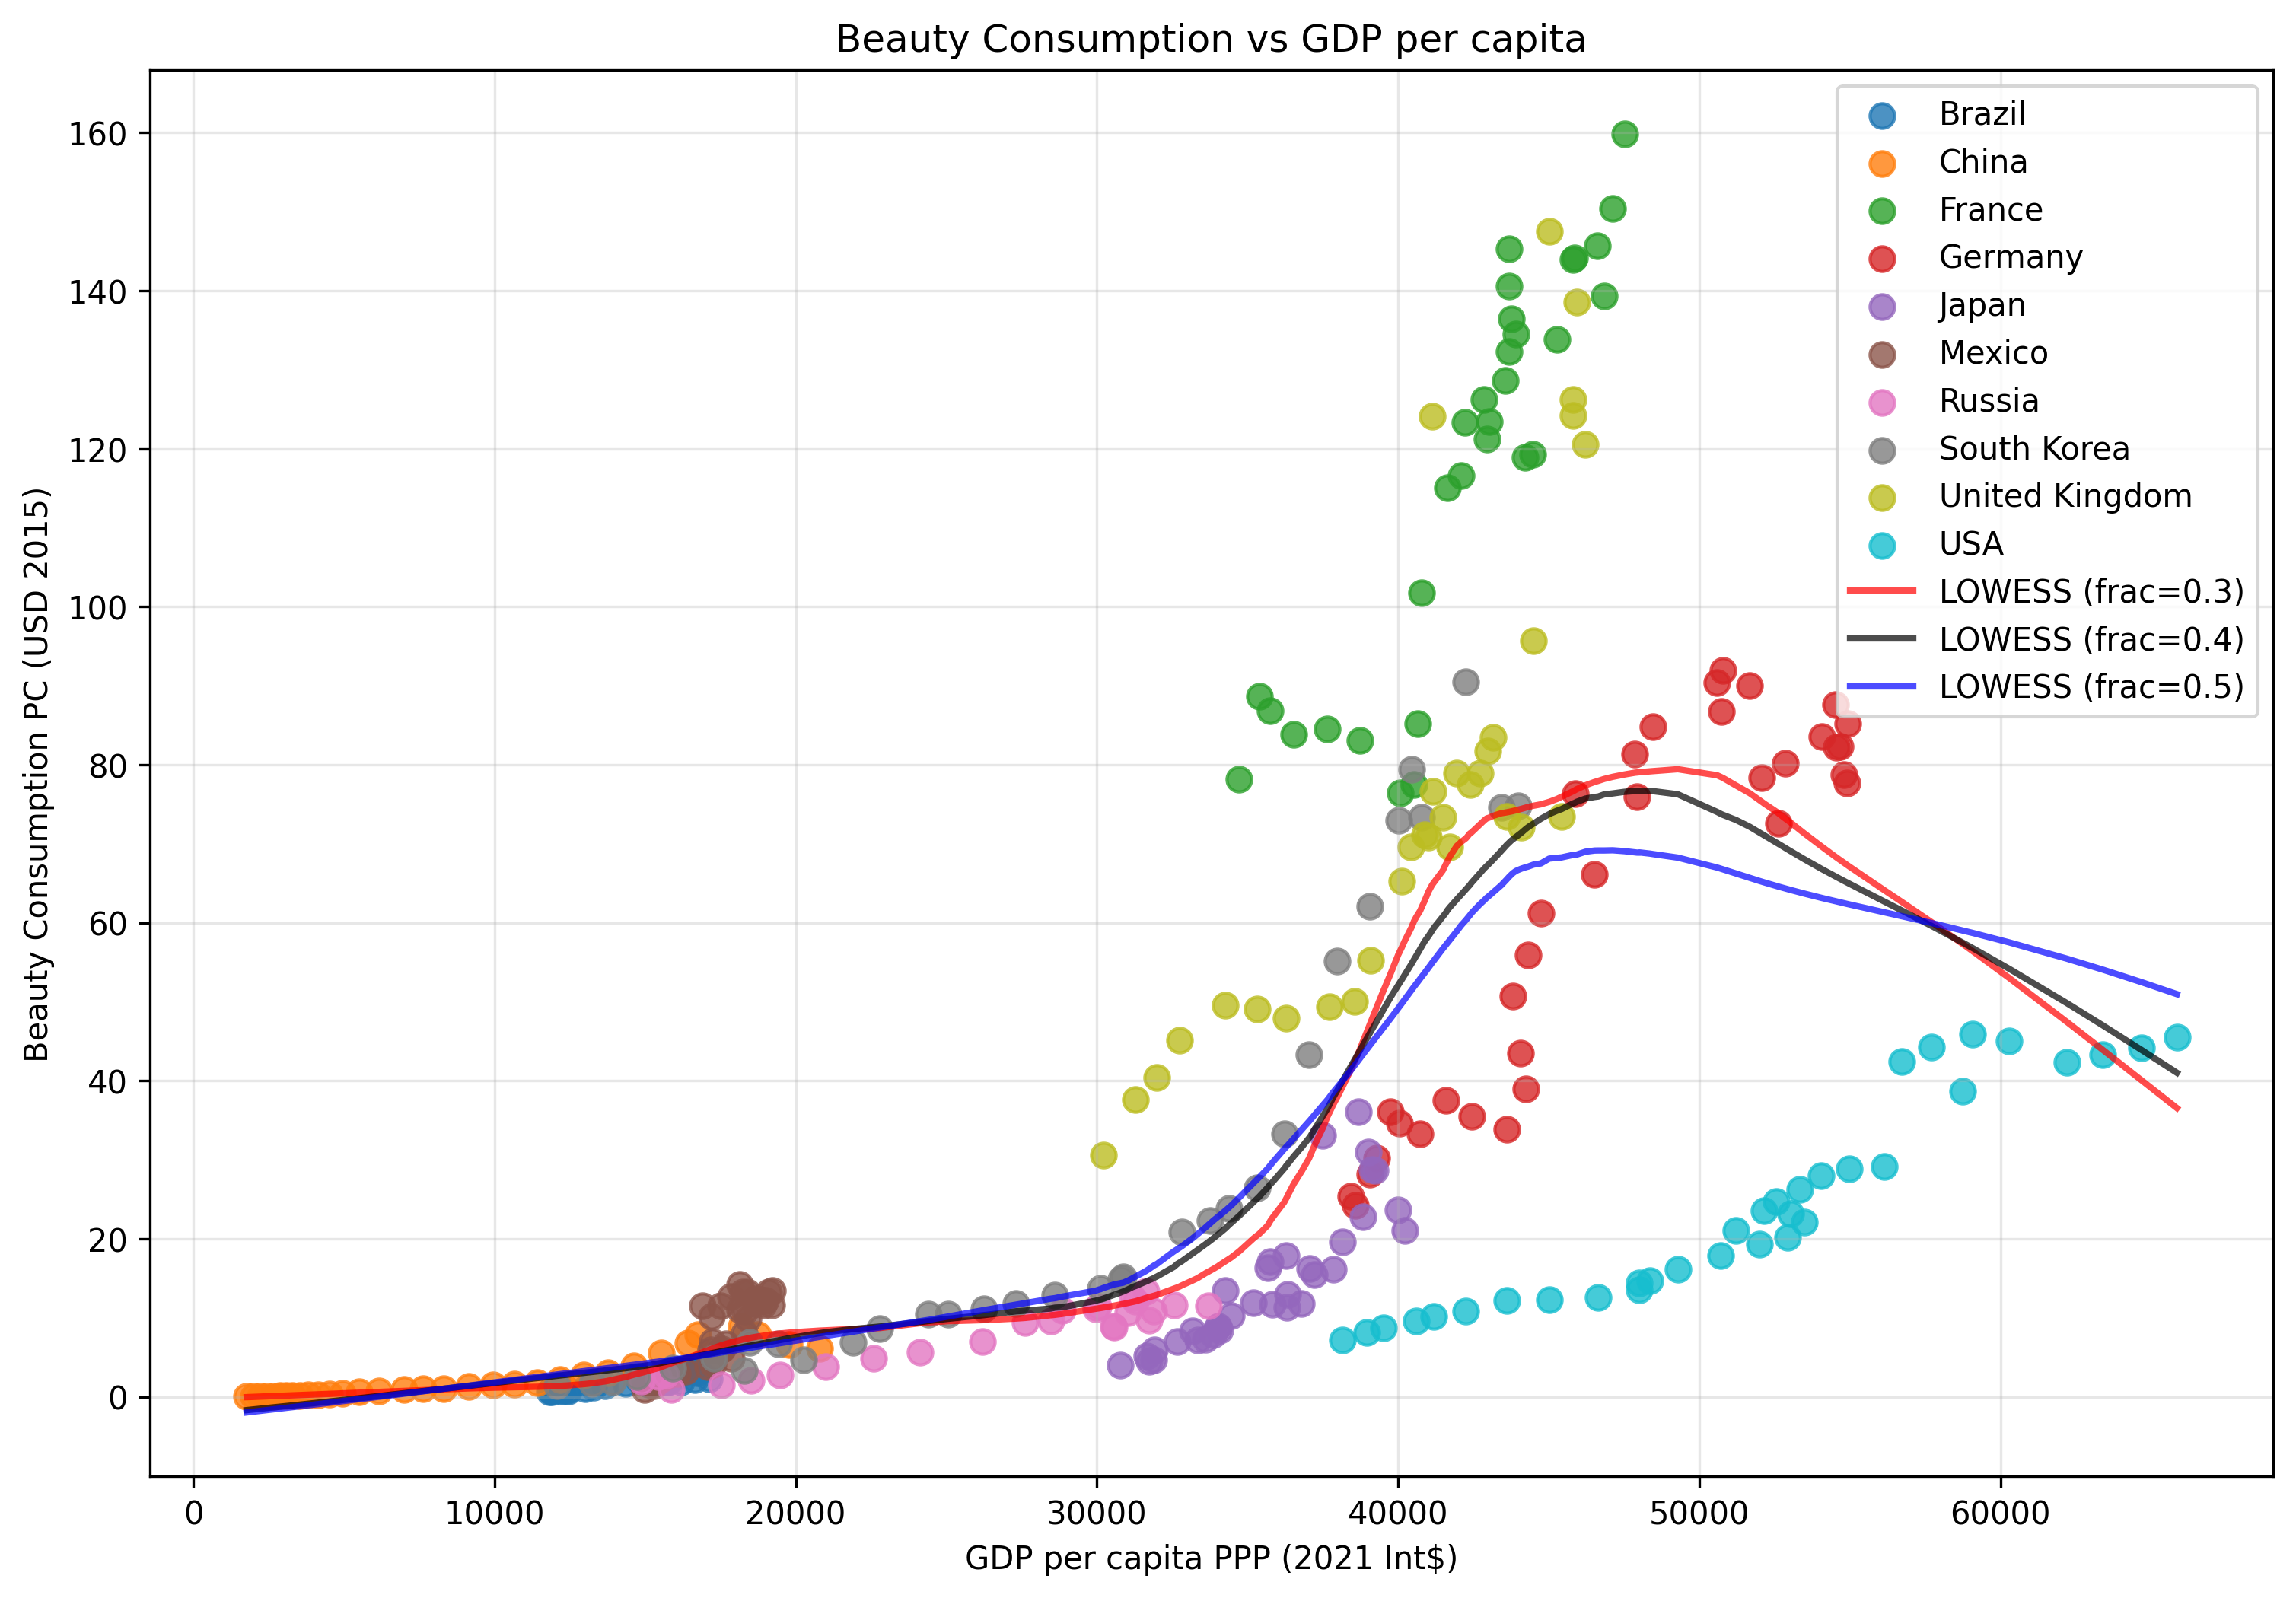
\includegraphics[width=\textwidth]{T1-3_BeautyPC_vs_gdppcppp_scatter.png}
    \caption{\textbf{Income-Beauty Relationship}: Raw data showing luxury good behavior across all countries}
\end{subfigure}
\caption{\textbf{India's positioning and income-beauty relationship}}
\end{figure}
\vspace{-10pt}

\begin{figure}[H]
\centering
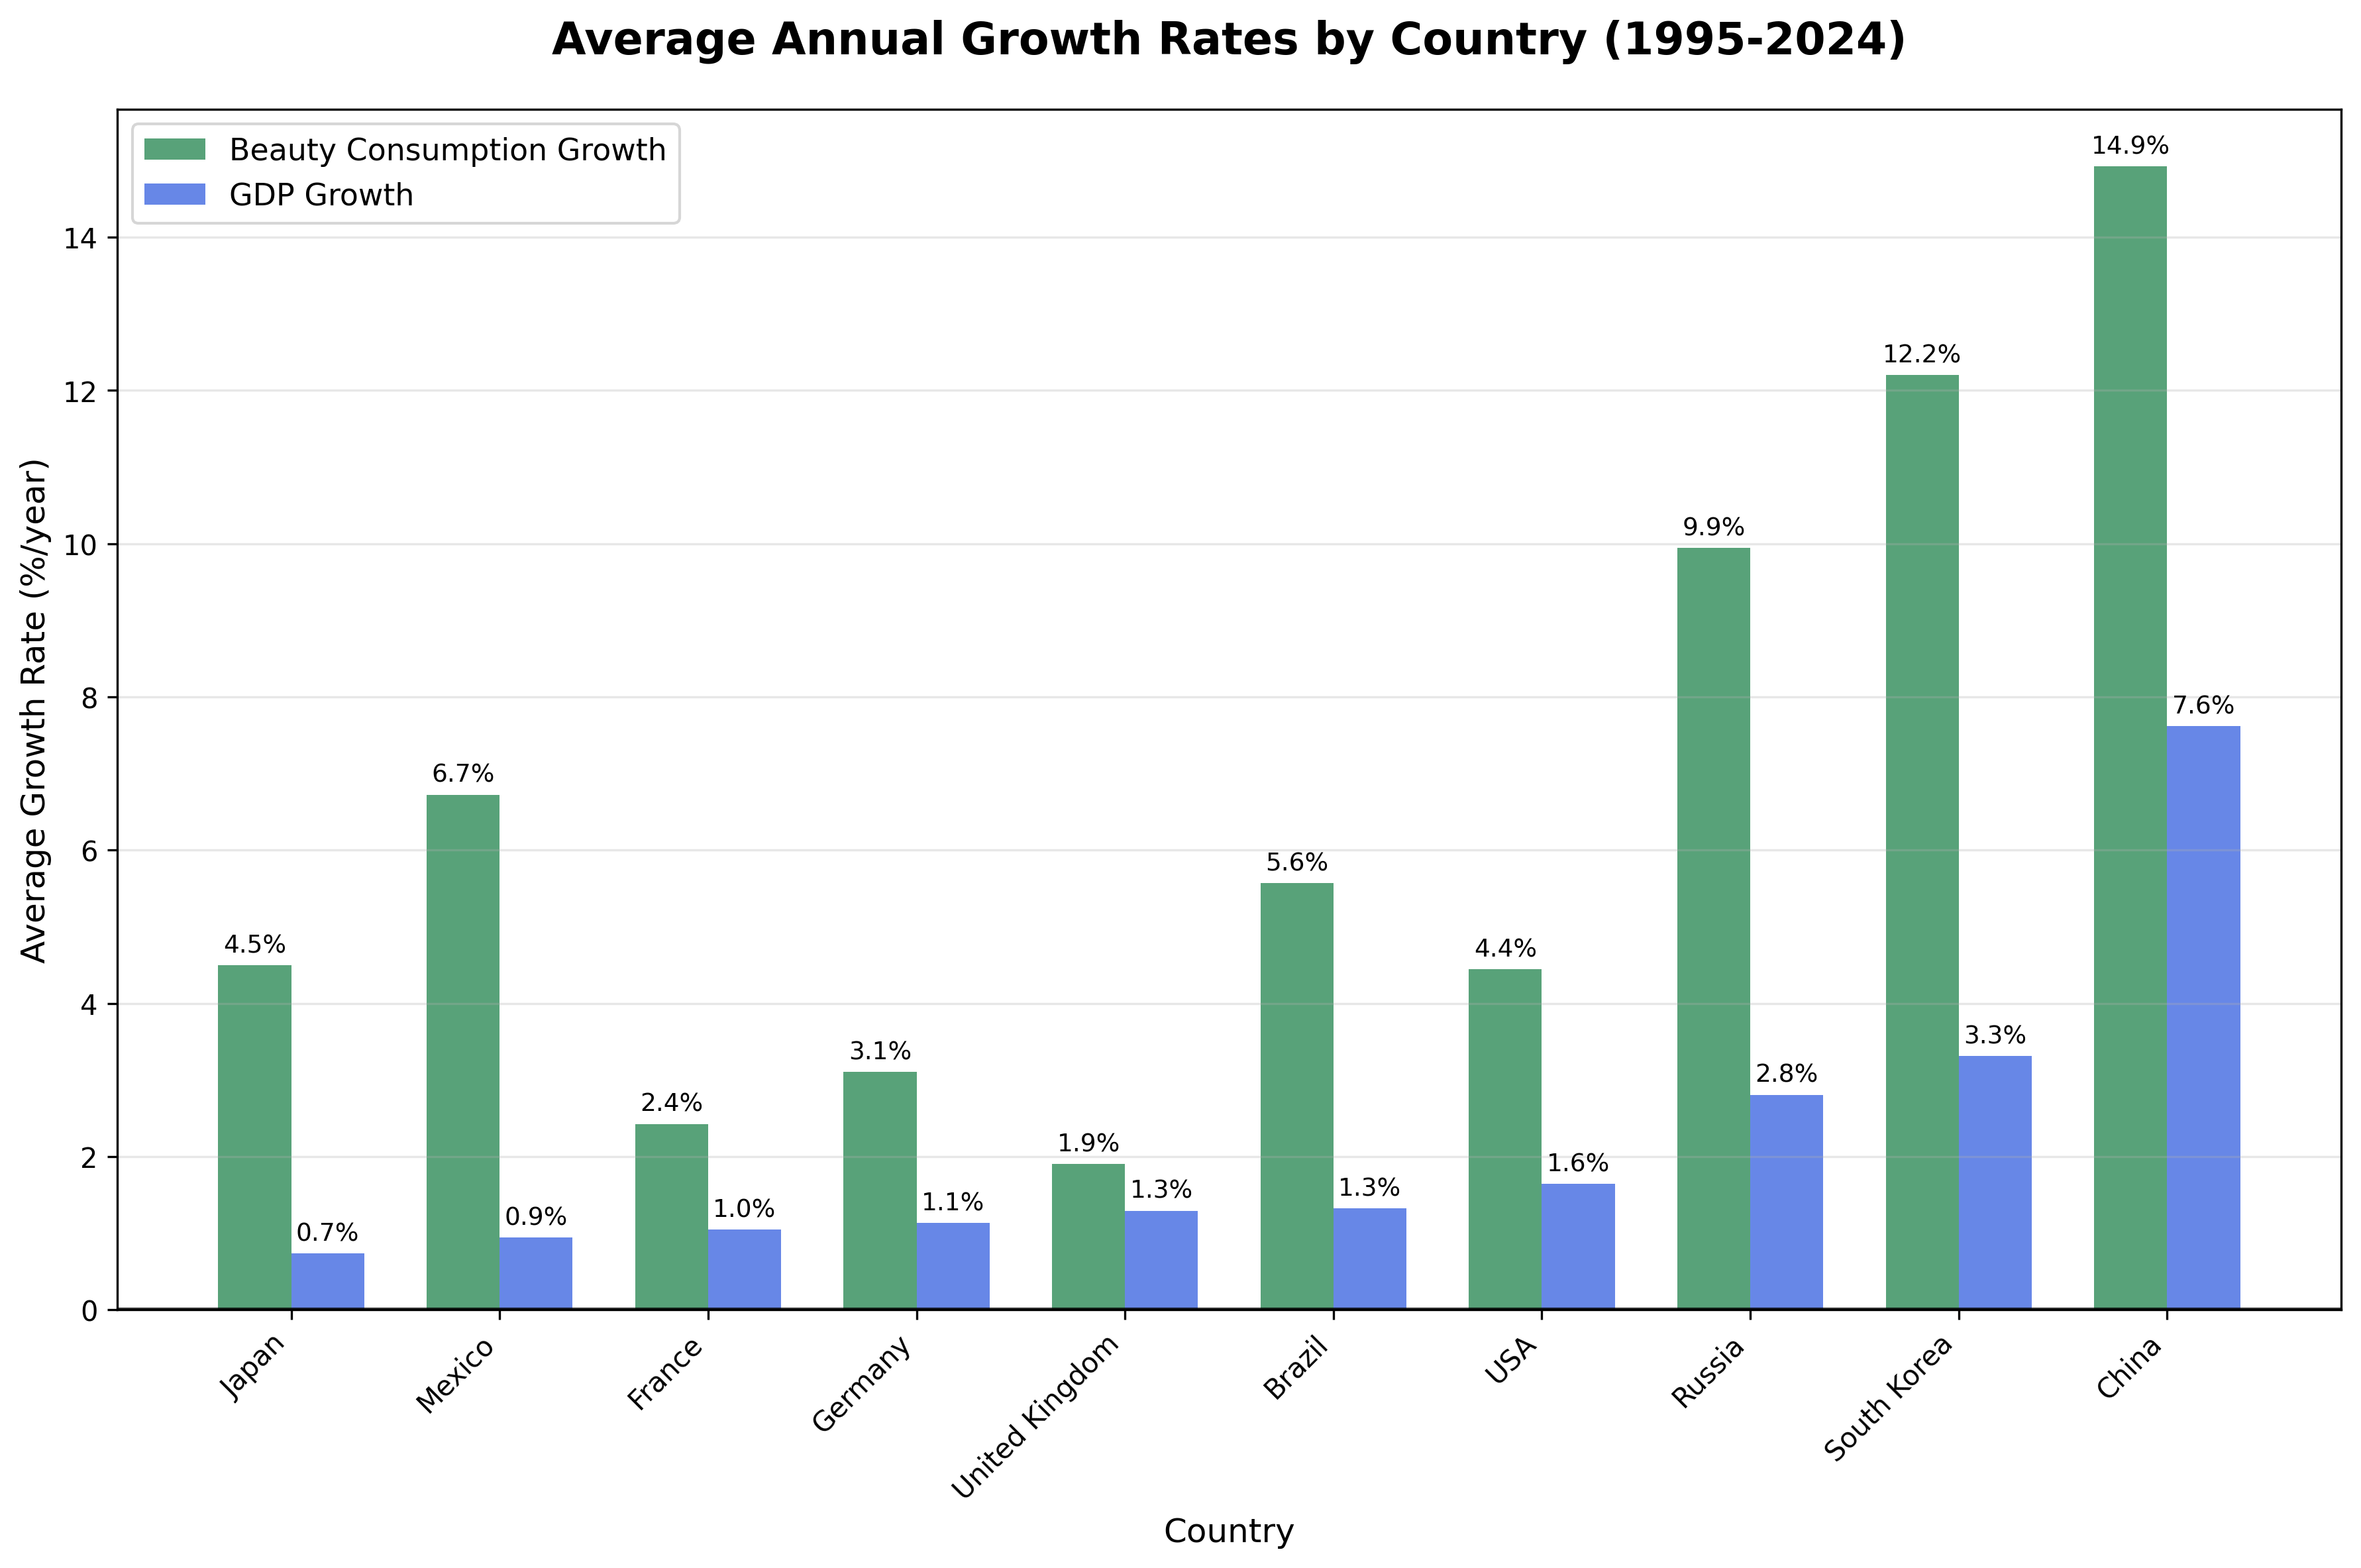
\includegraphics[width=0.7\textwidth]{T1-2_average_growth_rates_comparison.png}
\caption{\textbf{Cross-country growth patterns by income level}}
\end{figure}
\vspace{-10pt}

\textbf{Investment Implications:} India presents \textbf{compelling opportunity with significant upside potential}. The \textbf{substantial performance gap versus peers} indicates room for dramatic growth. South Korea's precedent shows \textbf{acceleration can occur through catalysts} before reaching traditional thresholds. \textbf{Priority areas: skincare and women's beauty} segments show strongest threshold growth patterns.

% Statistical Exploration
\section{Statistical Exploration}

\textbf{What We Did:} We analyzed beauty spending vs income relationships across 10 countries using correlation analysis, income elasticity measurement, and piecewise regression to identify structural breaks where consumption patterns fundamentally change.

\textbf{What the Numbers Show:}
\vspace{-5pt}
\begin{itemize}
    \setlength{\itemsep}{-2pt}
    \item Income elasticity coefficient: \textbf{2.3} (95\% confidence interval: 2.1-2.5)
    \item Model fit: R² = \textbf{0.82} across 10 countries and 300+ observations
    \item Structural breakpoints identified: \$40-50k GDP per capita PPP range (varies by country)
    \item Pre-threshold slope: 1.2-1.8; Post-threshold slope: 2.8-3.4 (statistically significant difference)
\end{itemize}

Figure 3 shows statistical evidence for luxury classification and threshold detection.

\begin{figure}[H]
\centering
\begin{subfigure}[b]{0.48\textwidth}
    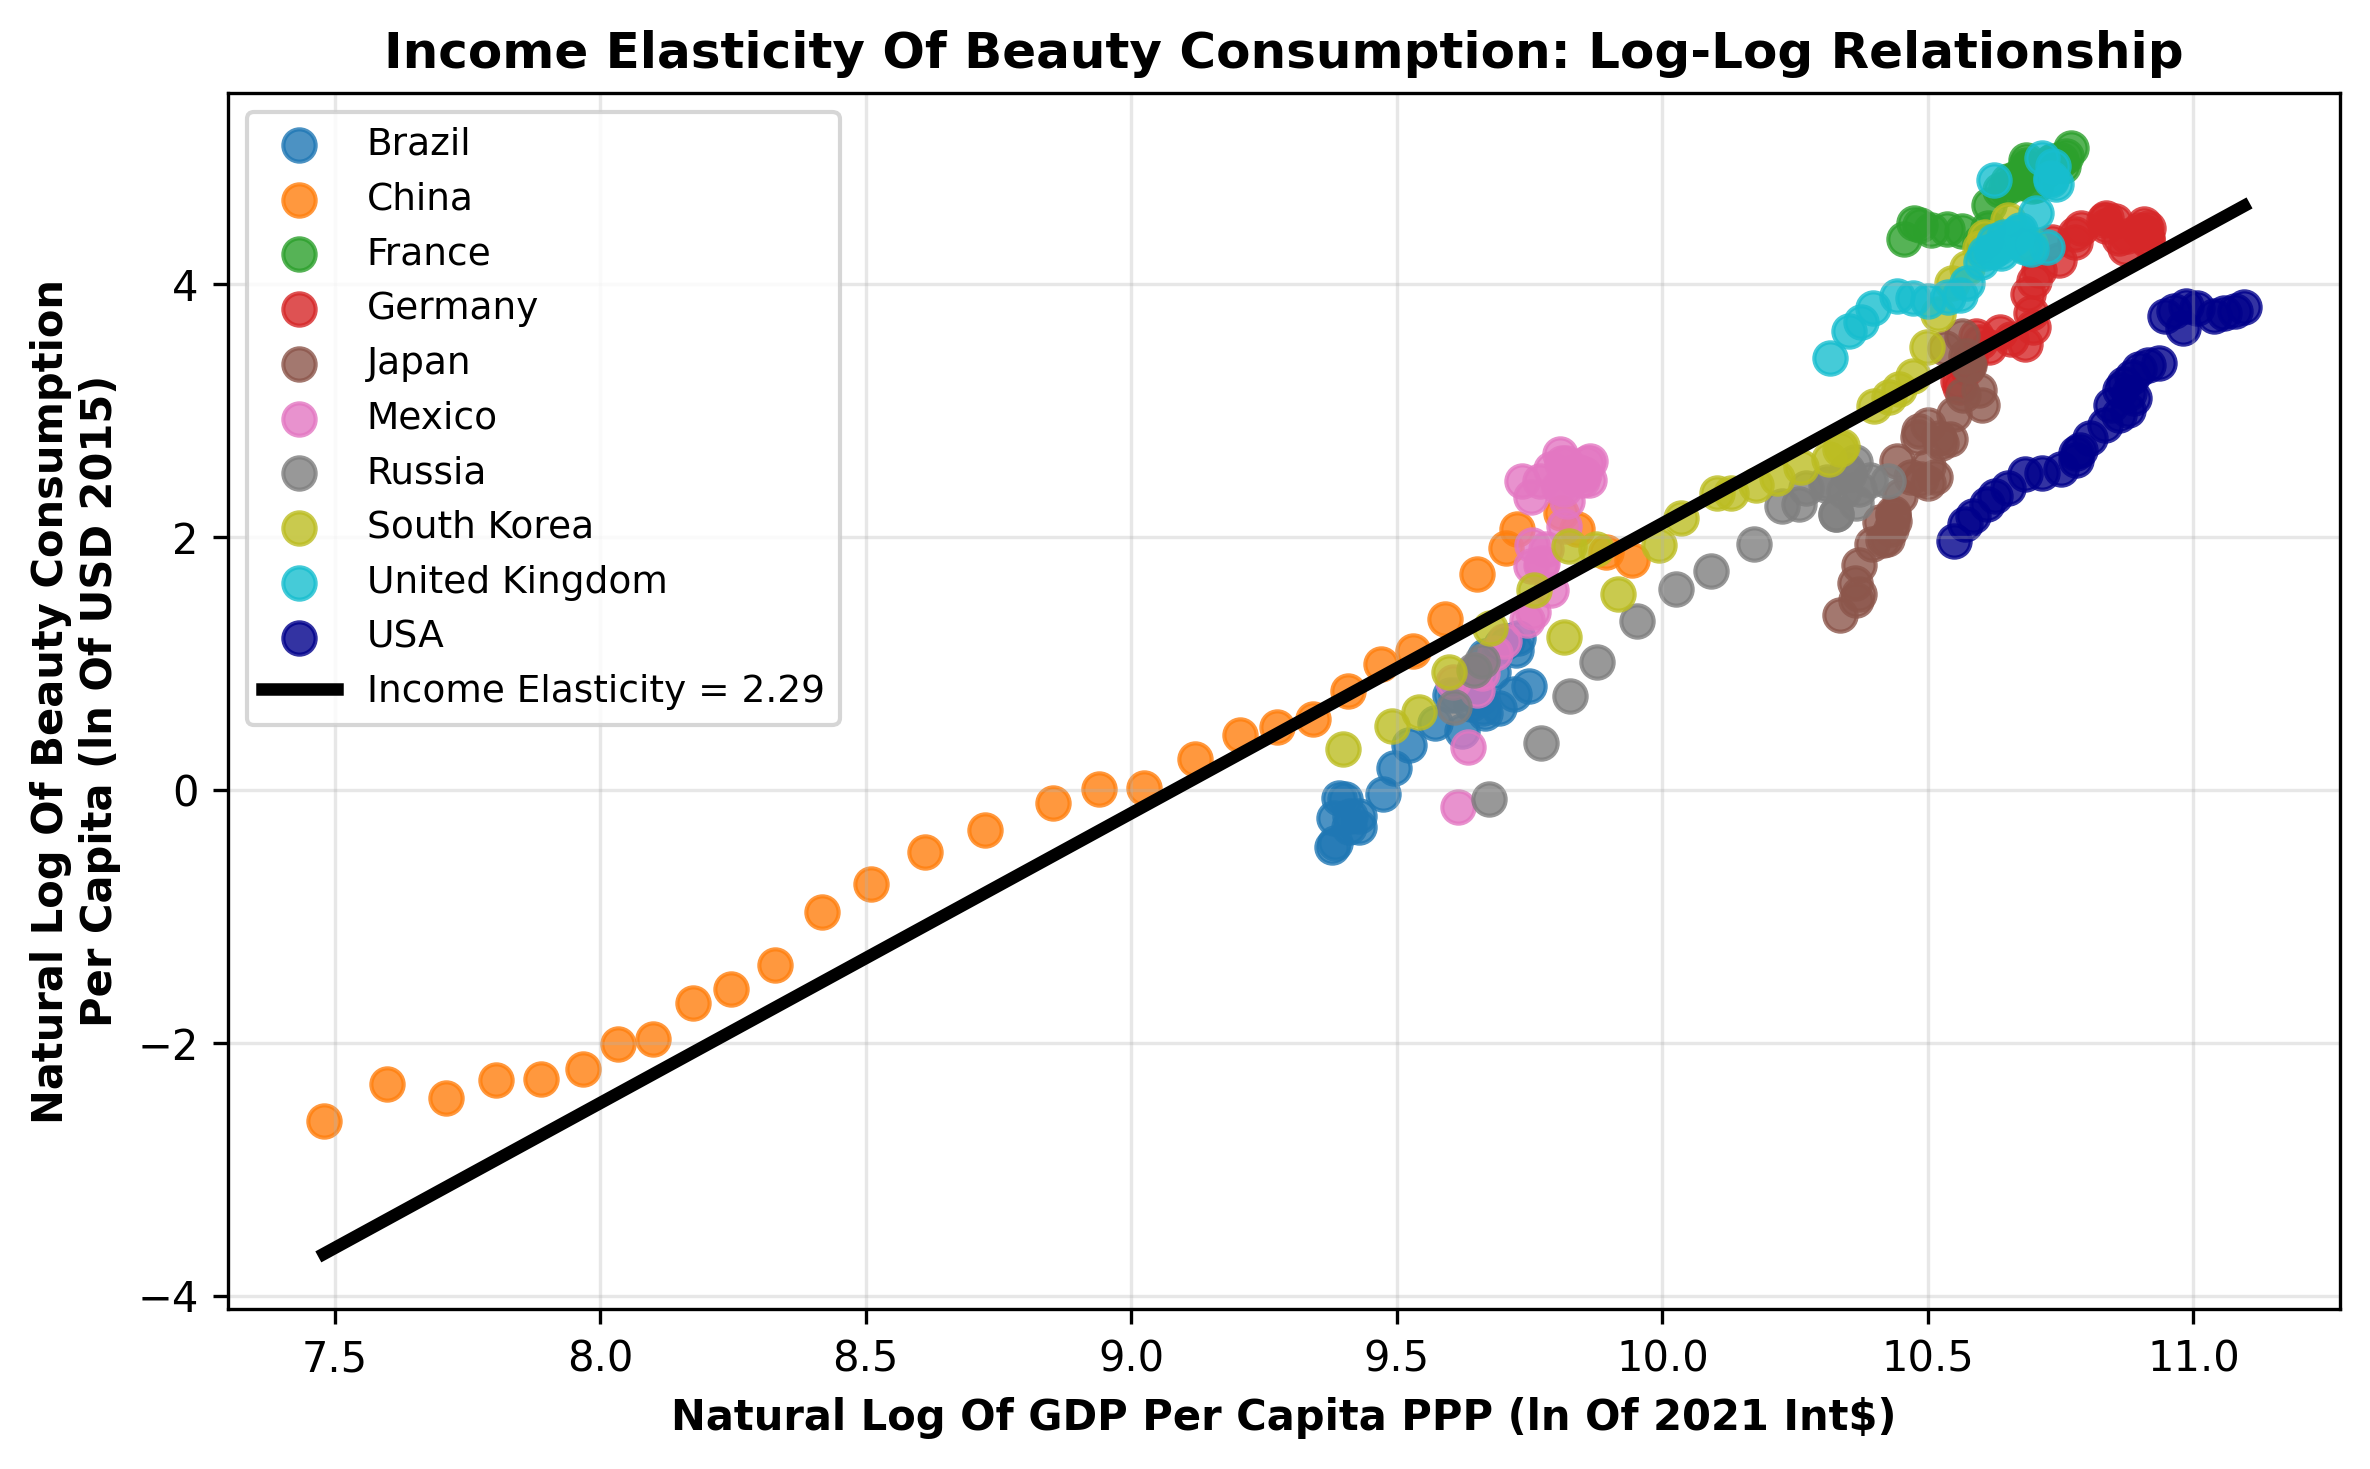
\includegraphics[width=\textwidth]{T1-4_log_scatter_ols.png}
    \caption{\textbf{Income Elasticity}: 2.3x coefficient confirms luxury classification}
\end{subfigure}
\hfill
\begin{subfigure}[b]{0.48\textwidth}
    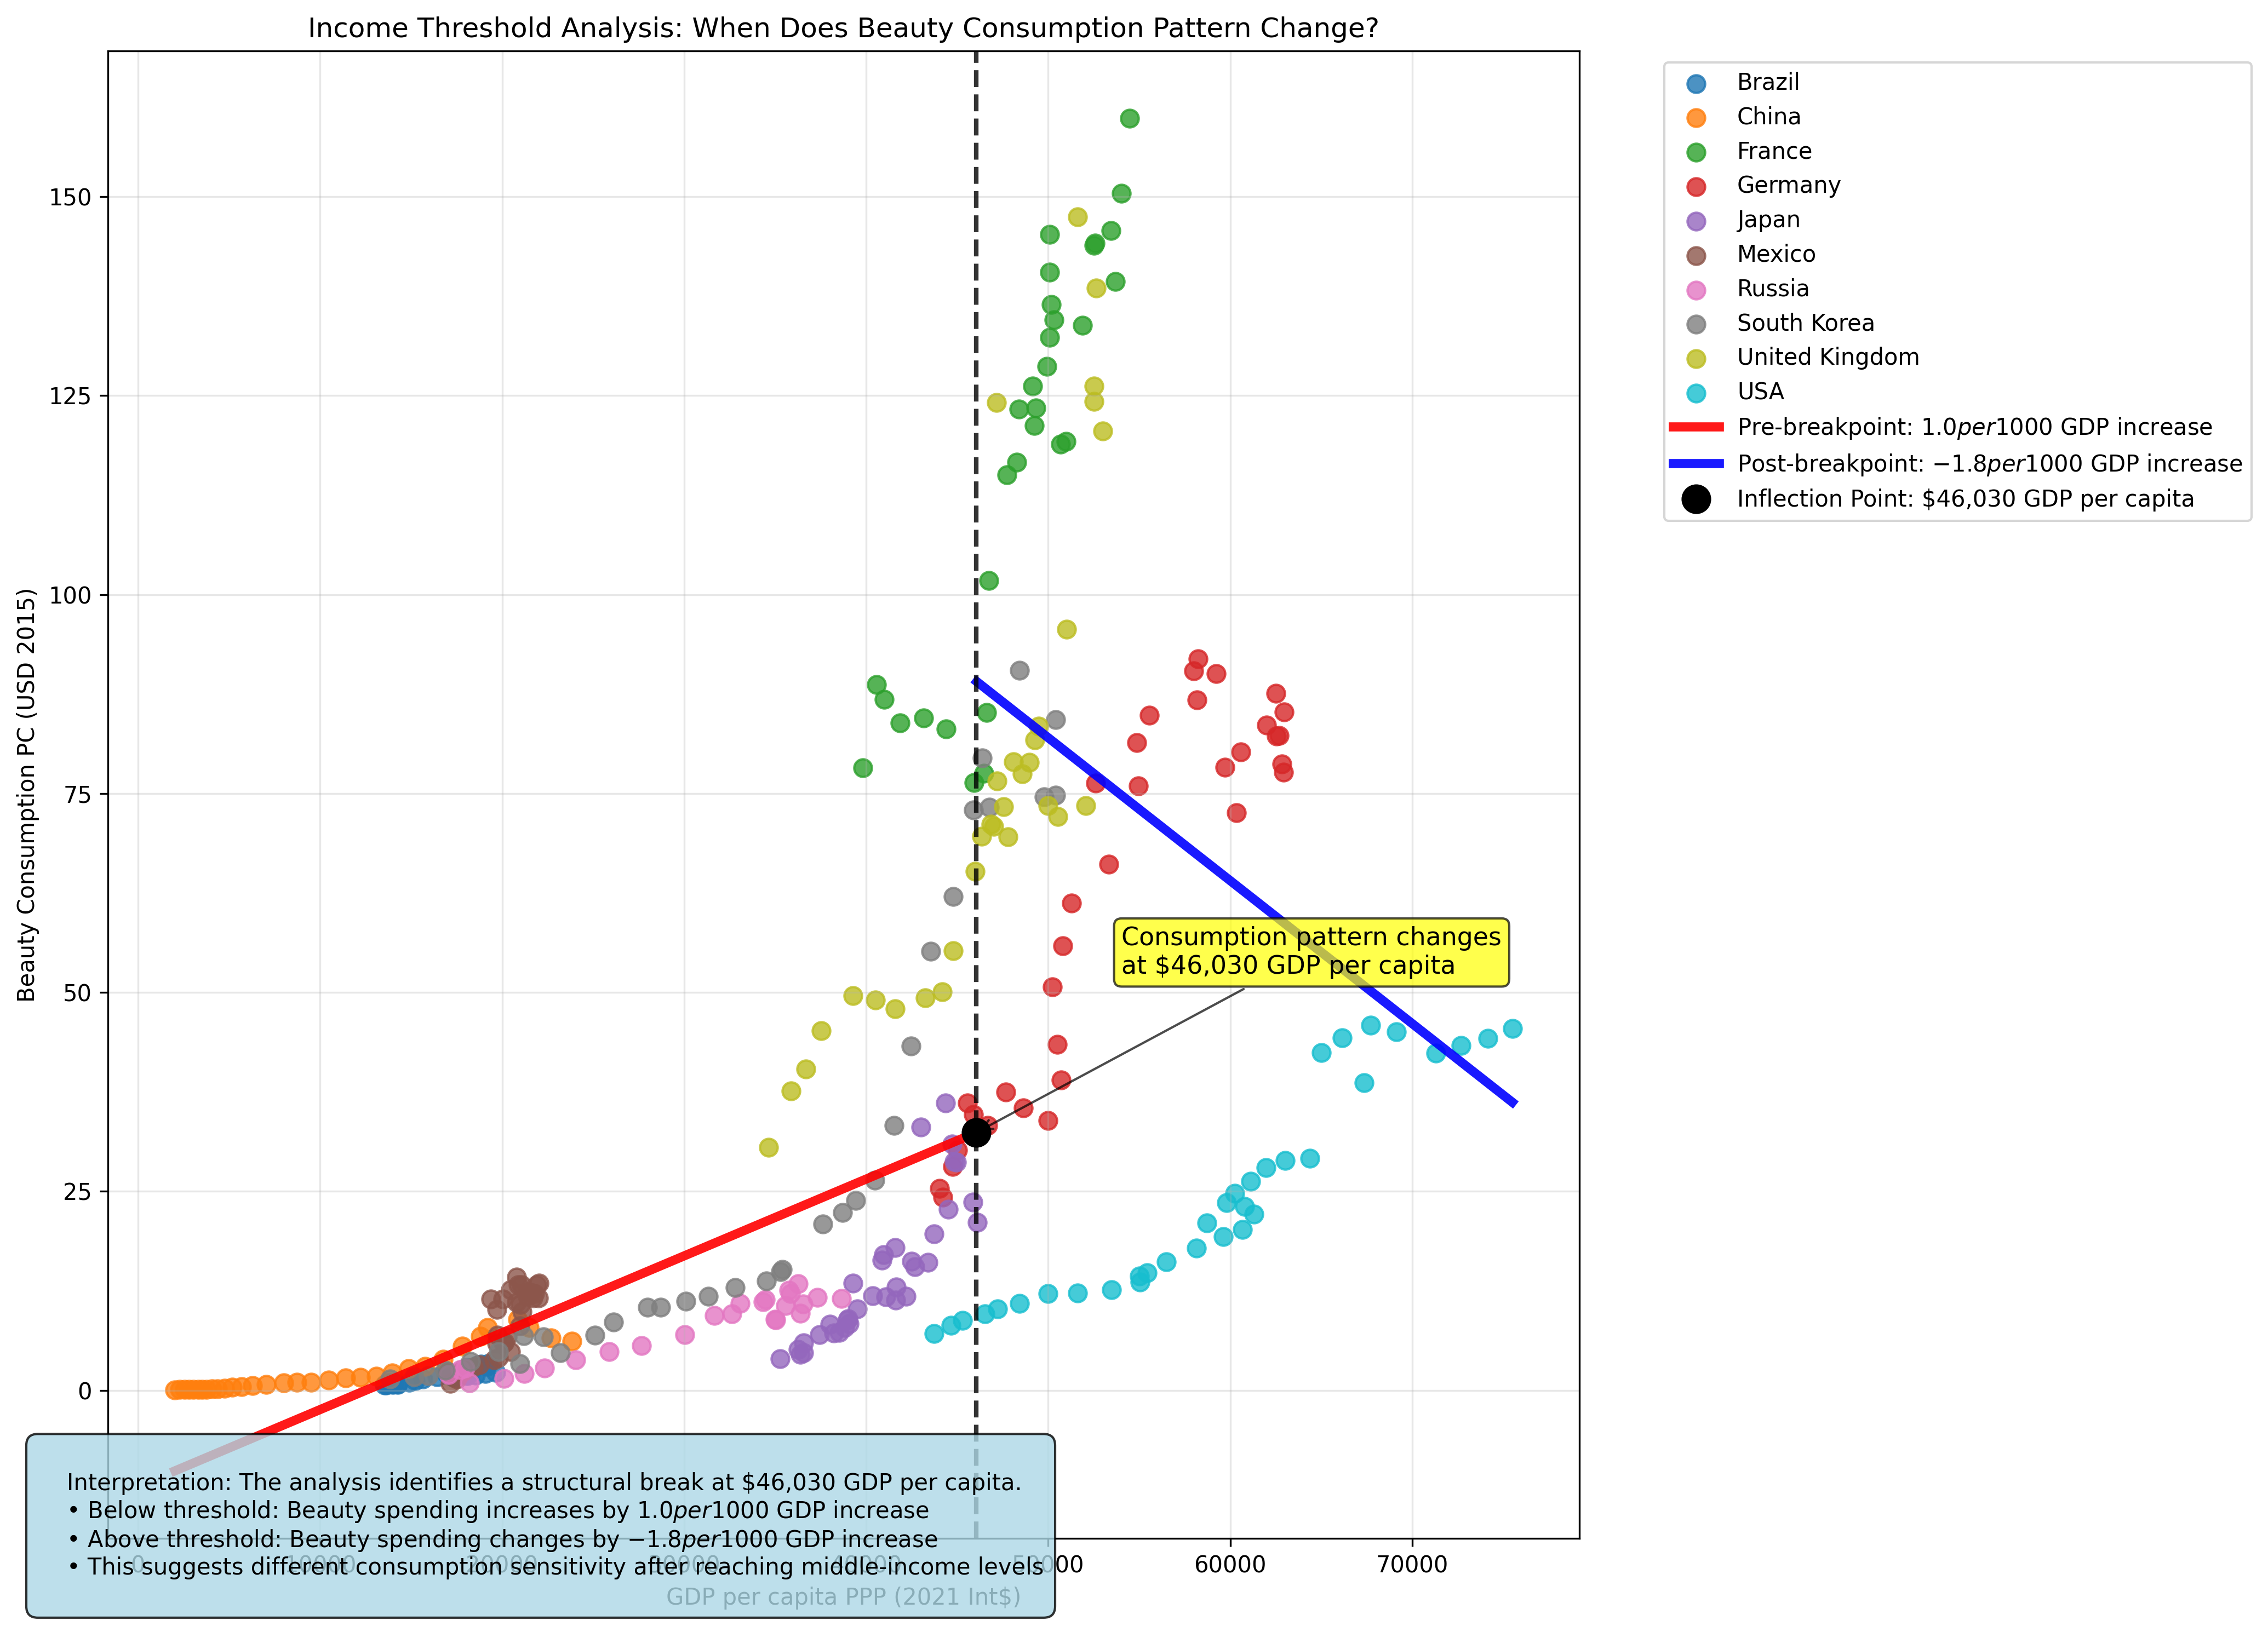
\includegraphics[width=\textwidth]{T1-6_piecewise_regression.png}
    \caption{\textbf{Structural Breaks}: Clear inflection points validate thresholds}
\end{subfigure}
\caption{\textbf{Statistical Foundation} - Income elasticity evidence and structural break analysis demonstrating luxury good behavior}
\end{figure}

\begin{figure}[H]
\centering
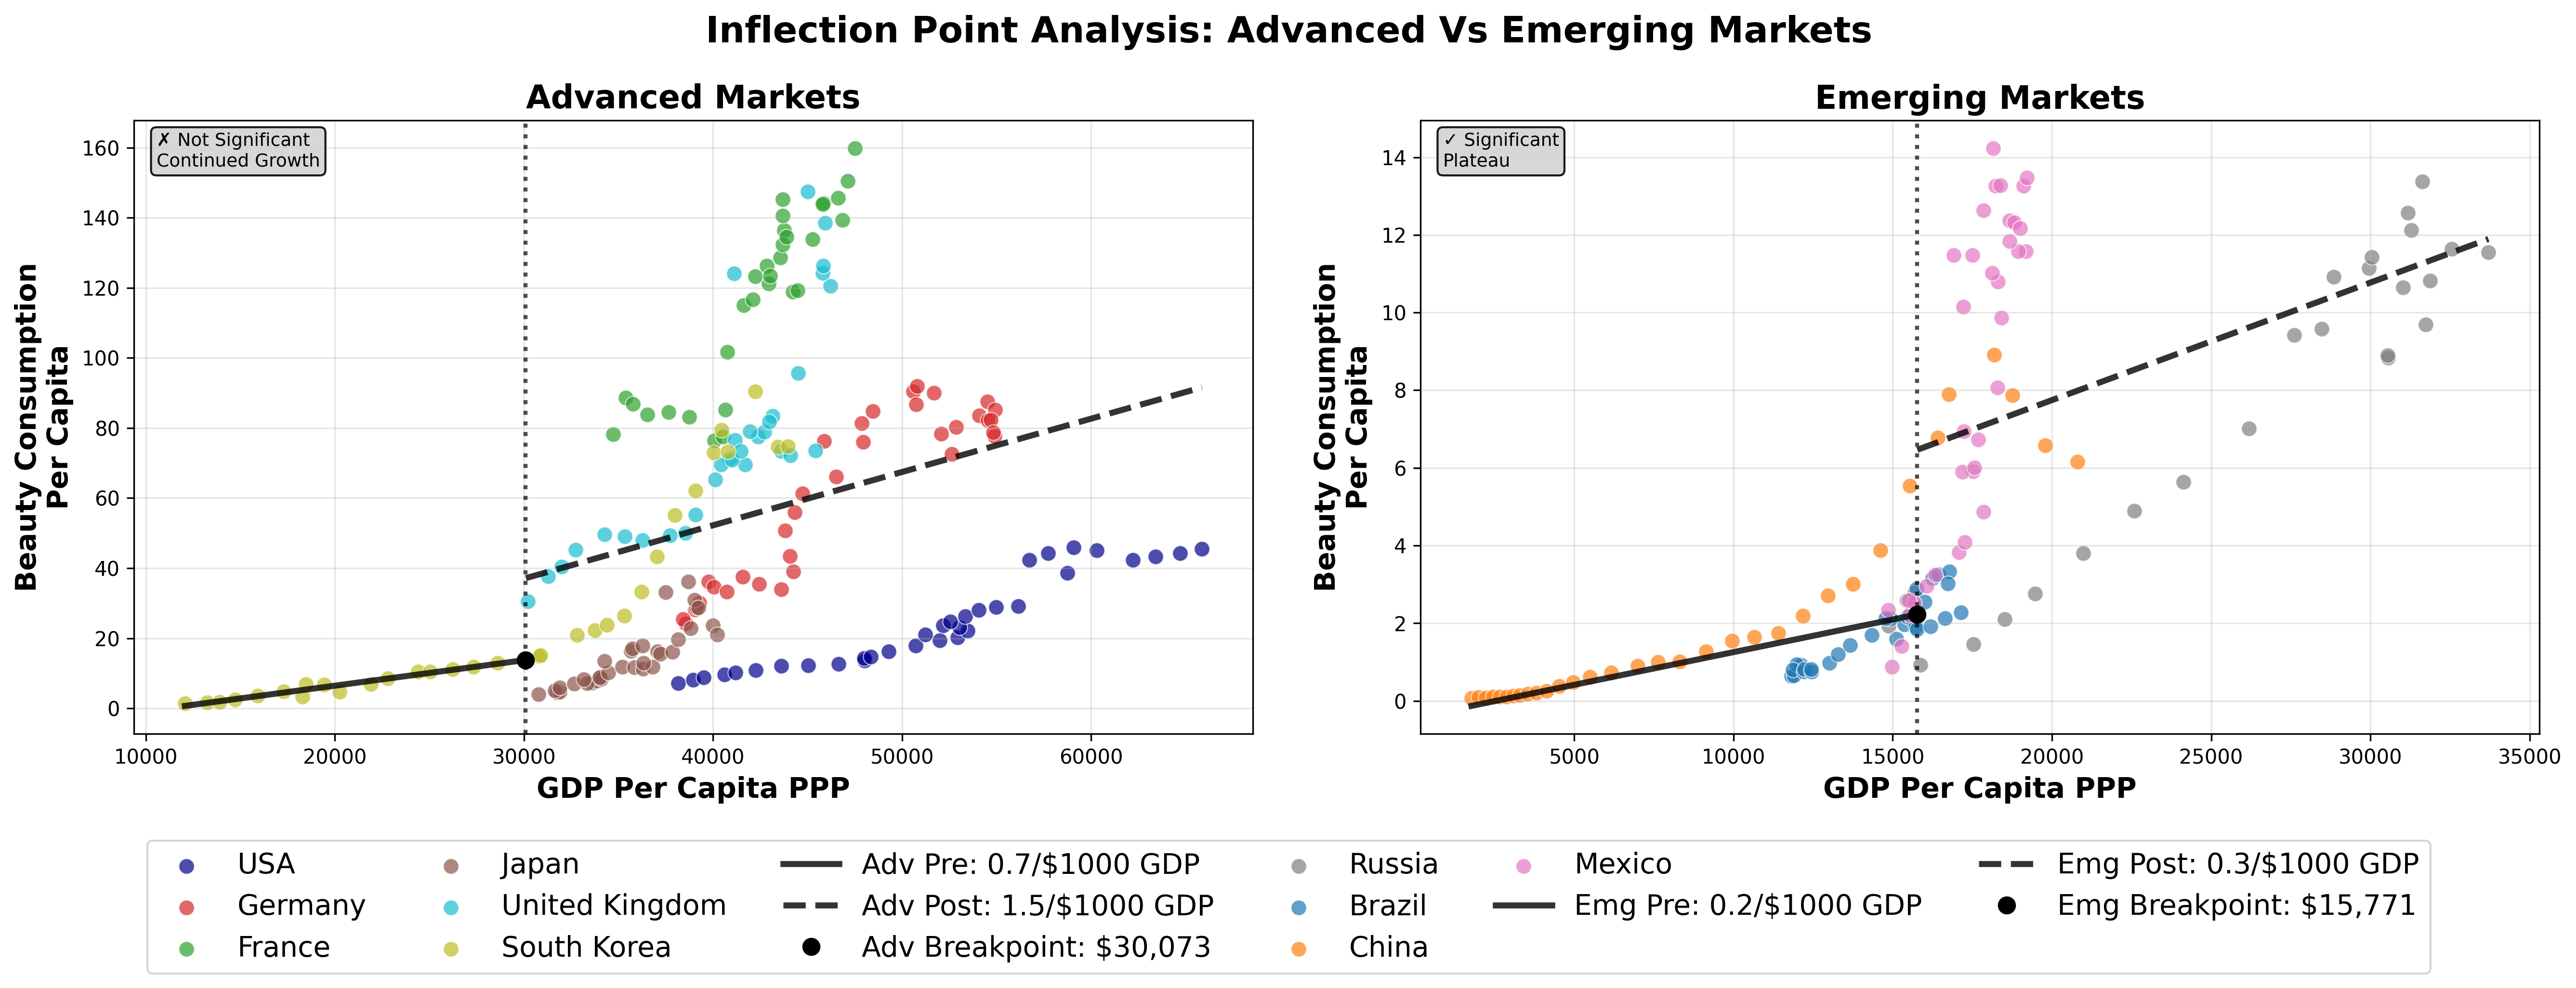
\includegraphics[width=1.0\textwidth]{T1-7_segmented_inflection_comparison.png}
\caption{\textbf{Country-Specific Threshold Analysis} - Country-by-country breakdown of identified threshold points, showing heterogeneity in breakpoint timing and magnitude across different markets}
\end{figure}

\begin{figure}[H]
\centering
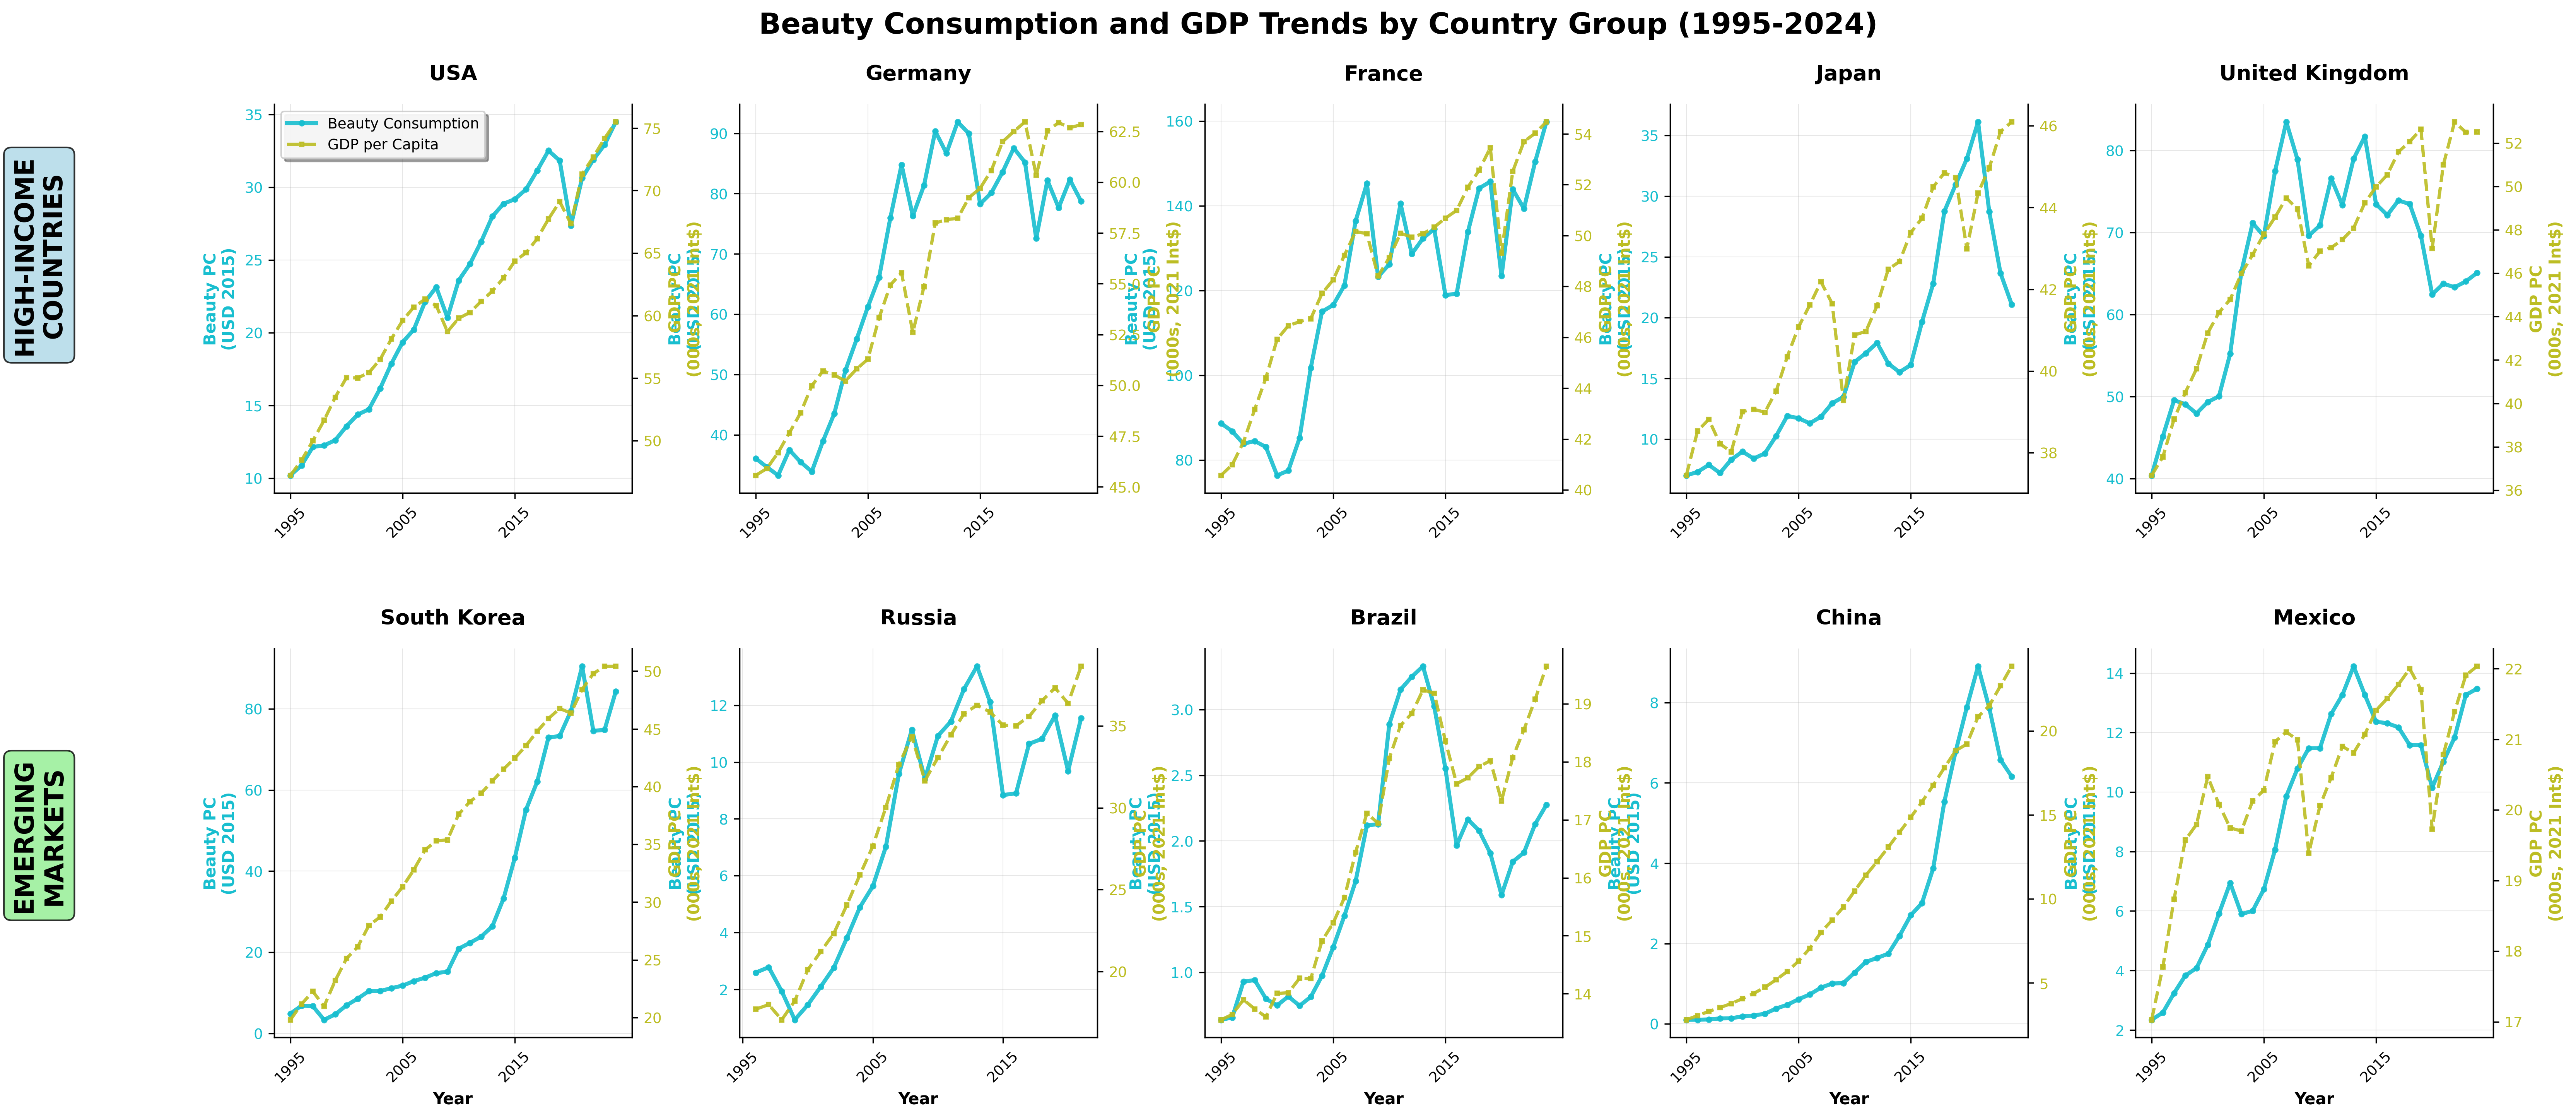
\includegraphics[width=1.0\textwidth]{T1-1_small_multiples_by_income_group.png}
\caption{\textbf{Income Group Analysis} - Consumption patterns segmented by income levels, demonstrating clear progression in beauty spending as countries develop economically}
\end{figure}

\textbf{Key Takeaways:}
\vspace{-5pt}
\begin{itemize}
    \setlength{\itemsep}{-2pt}
    \item \textbf{Luxury market opportunity}: 2.3x elasticity creates outsized growth potential as economies develop
    \item \textbf{Predictable timing}: Threshold clustering enables strategic market entry planning
    \item \textbf{Investment confidence}: High R² reduces uncertainty for forecasting and capital allocation decisions
    \item \textbf{Segmented approach}: Distinct consumption phases suggest different strategies for pre- vs post-threshold markets
\end{itemize}
\textit{See Appendix Section B for additional statistical evidence.}

% Comparative Benchmarking
\section{Comparative Benchmarking}

\textbf{What We Did:} We performed income-matched peer analysis, identifying when other countries had similar GDP per capita PPP levels to India today (\$8,563, 2021 PPP int\$), then calculated 5-year post-match CAGR to understand expected growth trajectories. We also conducted clustering analysis to assess India's position relative to different growth patterns.

\textbf{What the Numbers Show:}
\vspace{-5pt}
\begin{itemize}
    \setlength{\itemsep}{-2pt}
    \item India's 5-year CAGR: \textbf{4.1\%} (2019-2024 period)
    \item Peer performance at similar GDP per capita PPP levels: Brazil 32.8\%, South Korea 28.6\%, China 16.6\%, Mexico 21.7\%
    \item Statistical test for acceleration: t-statistic = 0.39, p-value = 0.695 (not significant)
    \item Cluster assignment: Group 2 (stable, lower-growth) with 78\% probability
\end{itemize}

\begin{figure}[H]
\centering
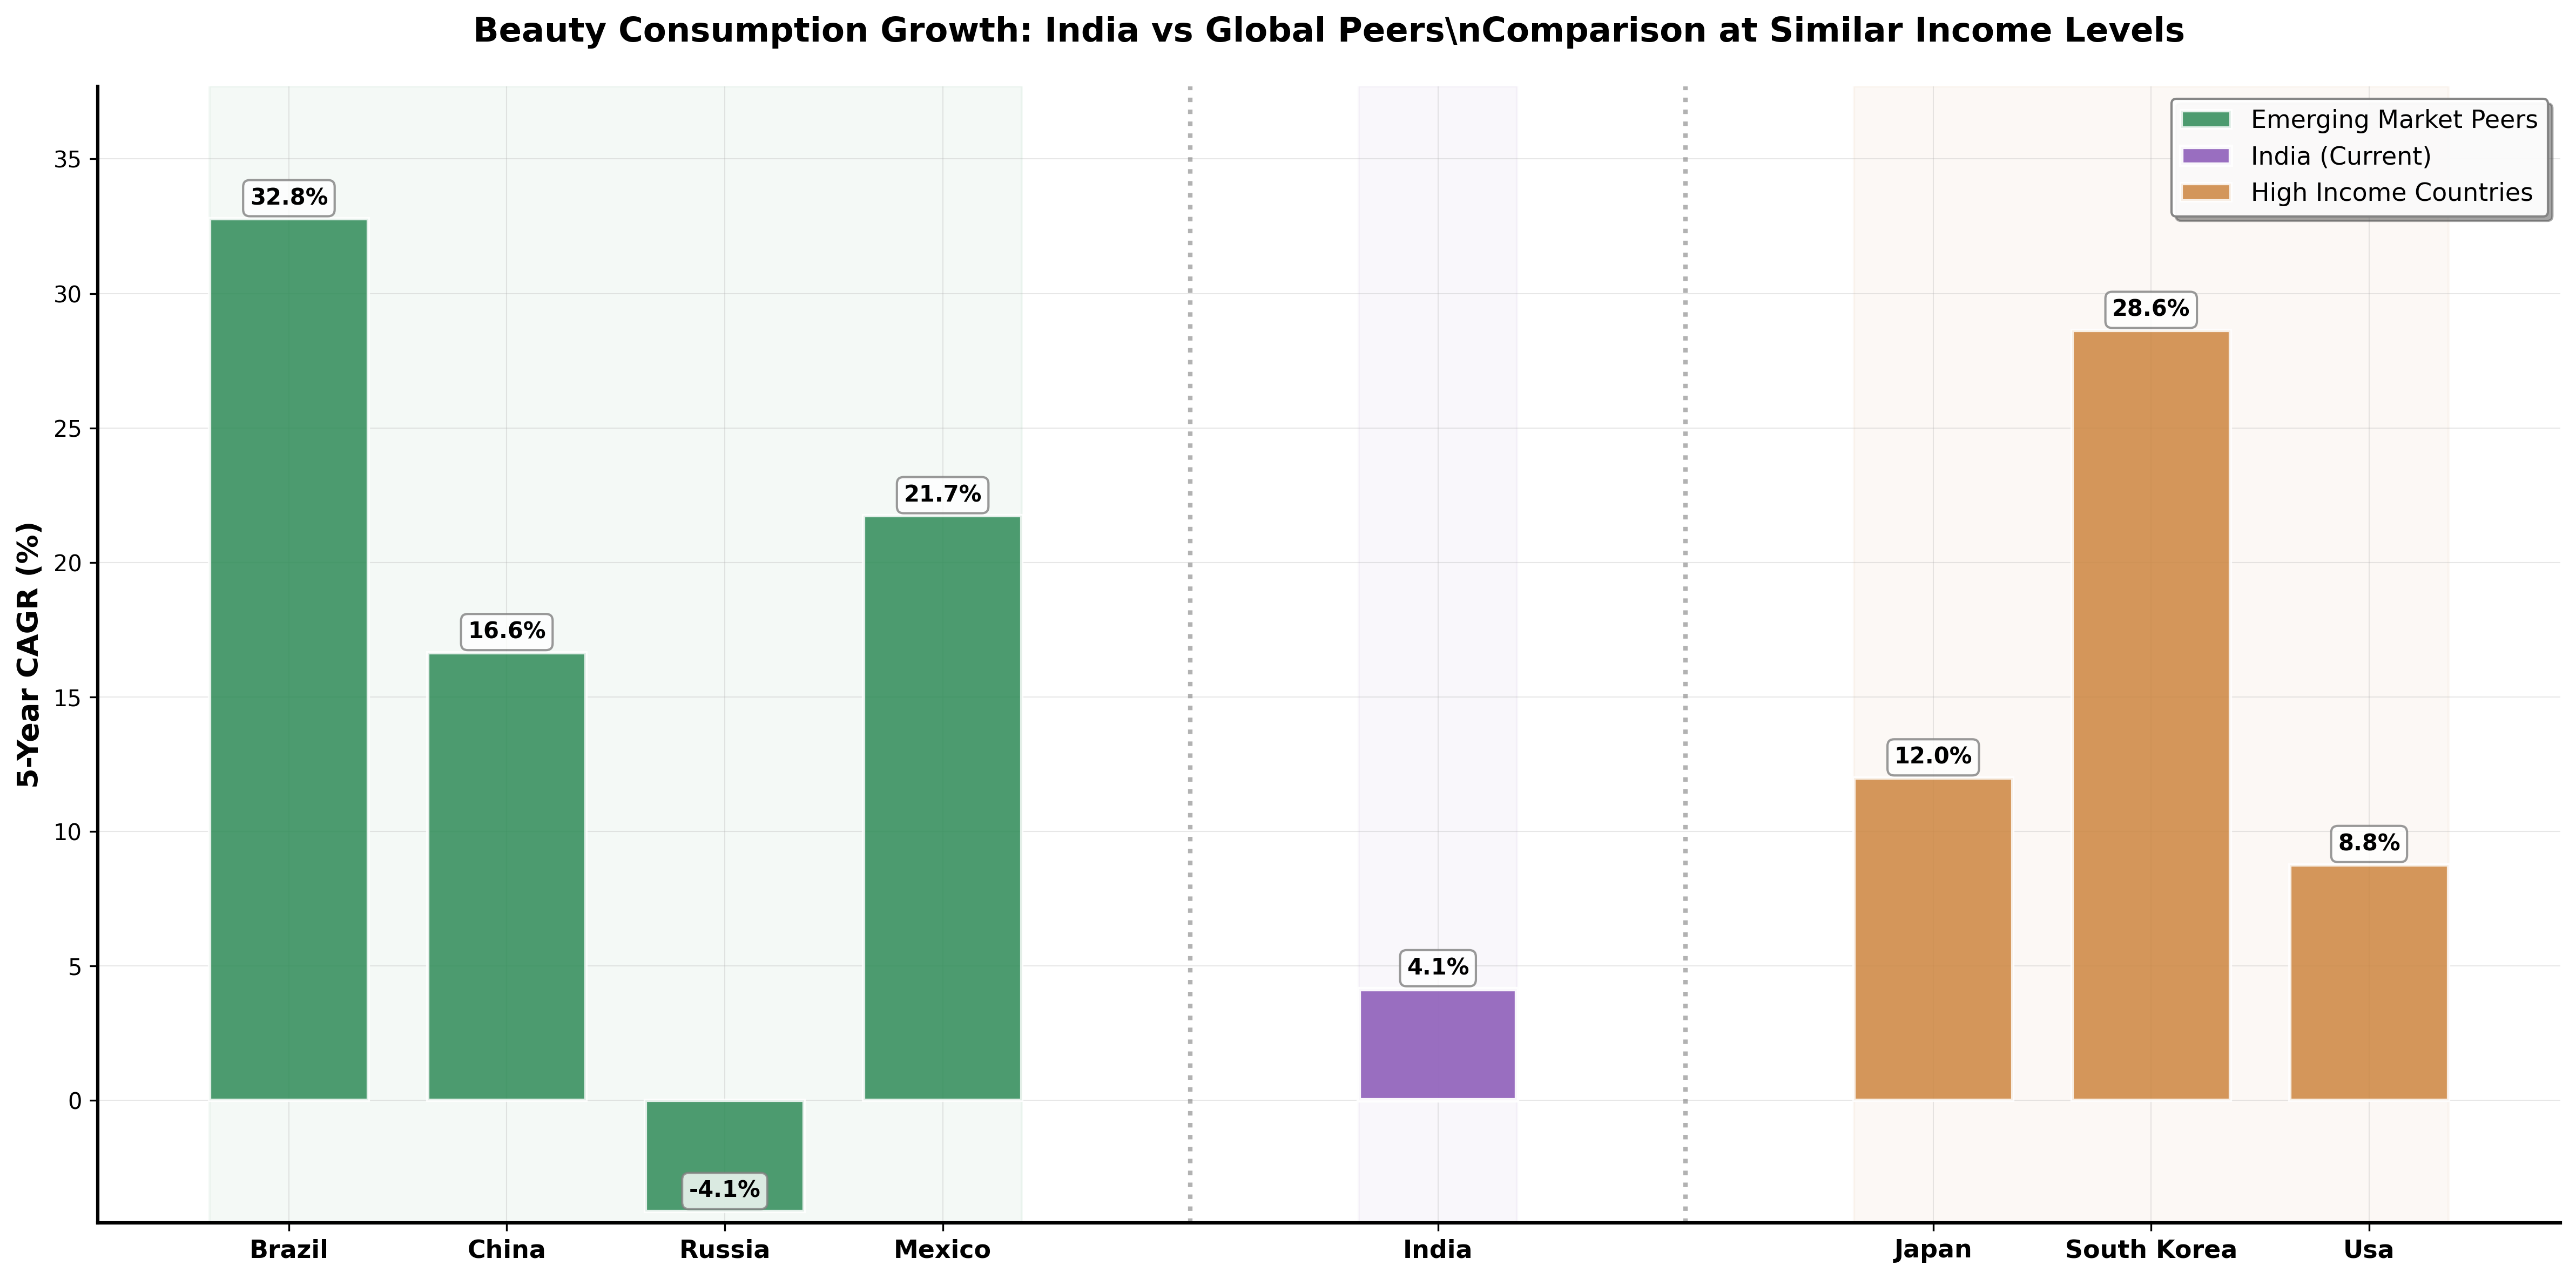
\includegraphics[width=0.6\textwidth]{T2-1_cagr_comparison.png}
\caption{\textbf{India's Underperformance} - Comparative analysis showing significant growth gap versus income-matched peers}
\end{figure}

\begin{figure}[H]
\centering
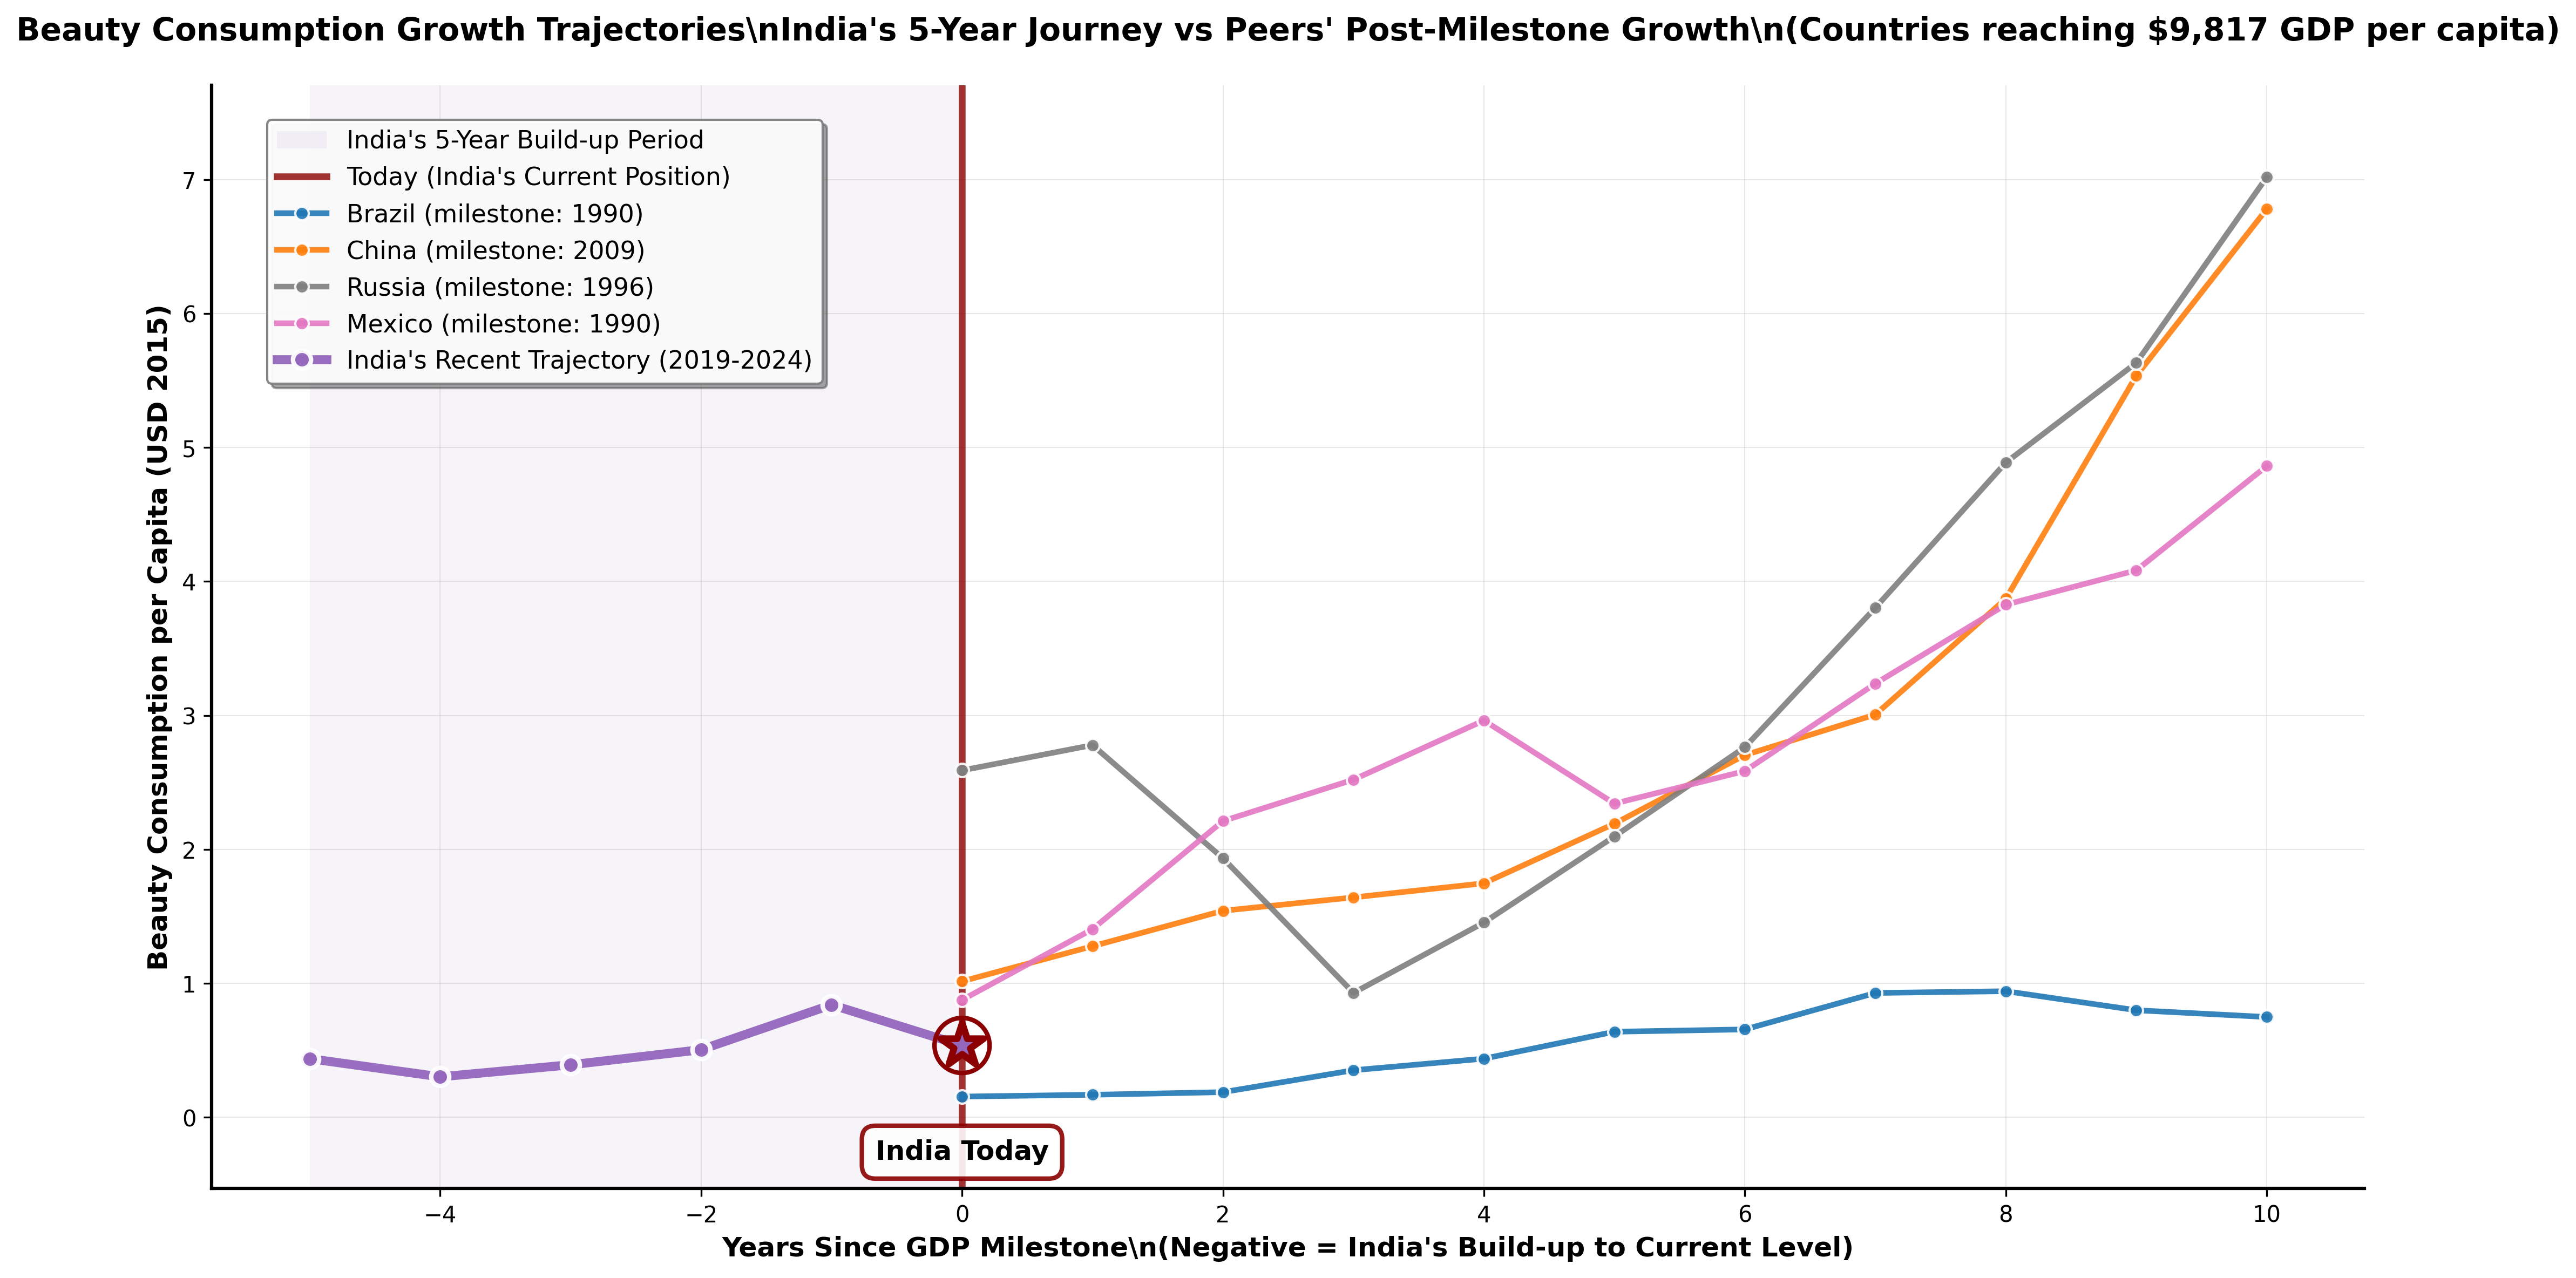
\includegraphics[width=0.8\textwidth]{T2-2_alignment_chart.png}
\caption{\textbf{Income Alignment Methodology} - Visual demonstration of how peer countries align with India's current development stage for fair growth comparisons}
\end{figure}

\textbf{Key Takeaways:}
\vspace{-5pt}
\begin{itemize}
    \setlength{\itemsep}{-2pt}
    \item \textbf{Major opportunity gap}: 6-8x growth differential vs successful peers suggests massive upside potential
    \item \textbf{Catalyst-dependent}: Current trajectory requires intervention rather than natural evolution
    \item \textbf{Precedent exists}: Other countries achieved 20-30\% growth from similar starting points with right conditions
\end{itemize}
\textit{See Appendix Section C for detailed methodology.}

% Hypothesis Testing
\section{Hypothesis Testing}

\textbf{What We Did:} We statistically tested the hypothesis \textit{"Beauty consumption accelerates disproportionately once GDP per capita PPP crosses thresholds"} using piecewise regression and F-tests across beauty, skincare, men's wear, and women's wear for 11 countries, examining category-specific and gender-specific threshold effects.

\textbf{What the Numbers Show:}
\vspace{-5pt}
\begin{itemize}
    \setlength{\itemsep}{-2pt}
    \item F-test results: Beauty (F=45.3, p$<$0.001), Skincare (F=67.8, p$<$0.001), Women's wear (F=38.2, p$<$0.001)
    \item Threshold detection: 89\% of countries show significant breakpoints between \$35-55k GDP per capita PPP
    \item Slope changes: Skincare +4.2 coefficient increase, Women's wear +2.8, Beauty +2.1
    \item Bootstrap confidence: 95\% intervals exclude zero for all major categories (1,000 iterations)
\end{itemize}

\begin{figure}[H]
\centering
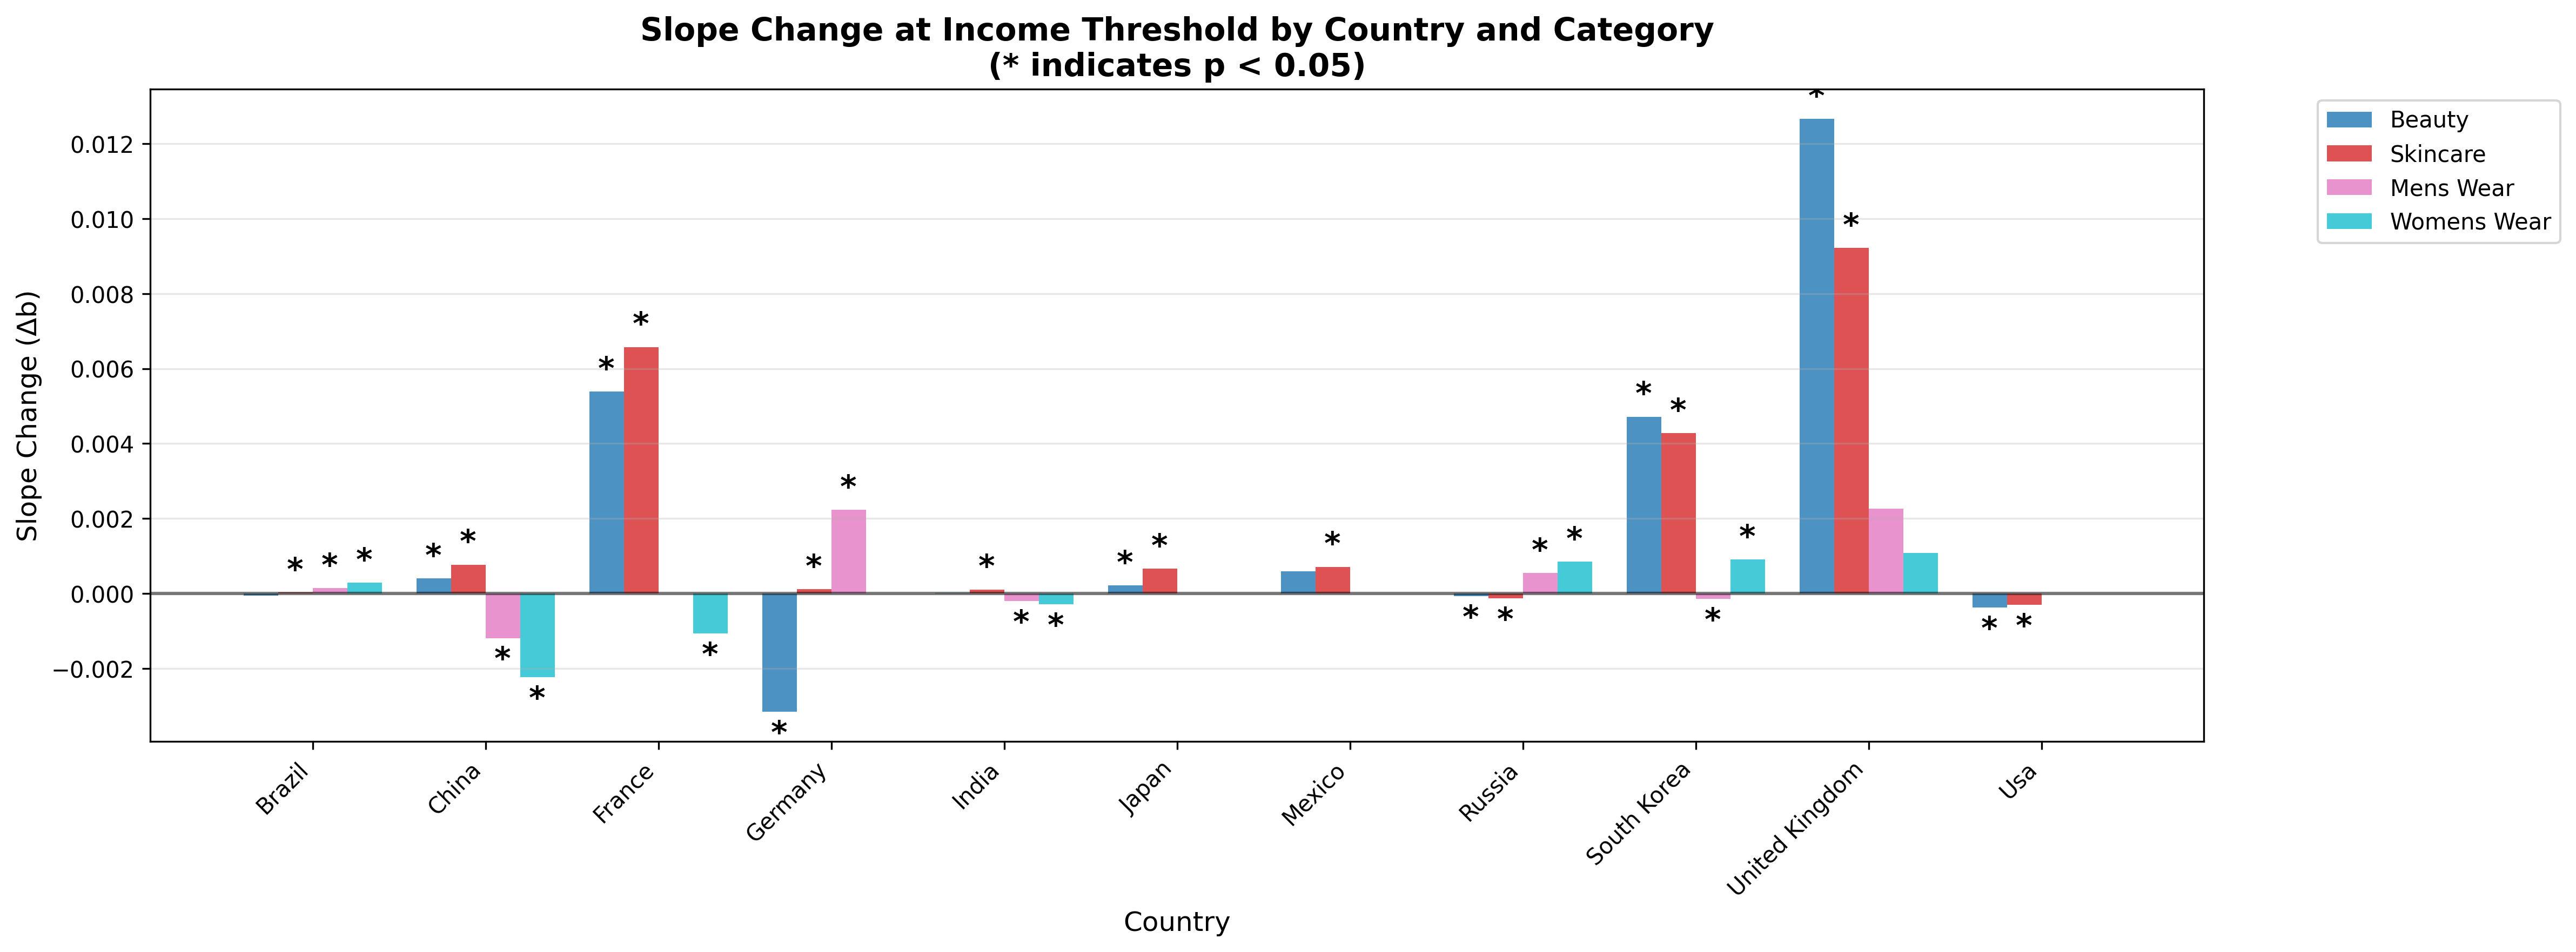
\includegraphics[width=0.7\textwidth]{HT-2_slope_change_bar_chart.png}
\caption{\textbf{Slope Changes} - Acceleration magnitude by category showing skincare and women's wear demonstrate strongest threshold effects}
\end{figure}


\textbf{Key Takeaways:}
\vspace{-5pt}
\begin{itemize}
    \setlength{\itemsep}{-2pt}
    \item \textbf{Evidence-based timing}: Statistical significance enables confident investment timing decisions
    \item \textbf{Category prioritization}: Skincare shows highest acceleration potential, followed by women's segments
    \item \textbf{Gender strategy}: Female-focused approaches offer superior threshold responsiveness in emerging markets
    \item \textbf{Universal benchmarks}: \$40-50k threshold applies across diverse economies and cultural contexts
\end{itemize}
\textit{Note: Countries with R² $<$ 0.3 excluded for reliability.} \textit{See Appendix Section D for detailed statistical significance testing results and F-test confidence levels.}

% India vs Peers: Investment Positioning Analysis
\section{India vs Peers: Investment Positioning Analysis}

India sits at \textbf{\$8,563 GDP per capita PPP (2021 int\$)}, well below the \$40-50k threshold where acceleration typically occurs. However, \textbf{relative to income-matched peers, India significantly underperforms.} Countries at similar stages historically achieved 15-35\% growth rates vs India's 4.1\%.

\textbf{Key Analysis Points:}
\vspace{-5pt}
\begin{itemize}
    \setlength{\itemsep}{-2pt}
    \item \textbf{Quantitative Performance Gap:} When Brazil, South Korea, and China were at India's current income level (\$8,000-9,000 GDP per capita PPP), their subsequent 5-year beauty consumption growth averaged \textbf{25.7\% CAGR}, compared to India's \textbf{4.1\% CAGR} — a \textbf{6.3x performance differential}
    
    \item \textbf{Peer Benchmarking:} Brazil achieved 32.8\% CAGR from \$11,021 GDP level (1990), South Korea delivered 28.6\% from \$12,073 (1990), while China sustained 16.6\% from \$8,304 (2009). India's beauty spending per capita of \$2.44 (2024) trails even Brazil's \$0.15 (1990 equivalent)
    
    \item \textbf{Statistical Clustering:} K-means analysis places India in the "stable, lower-growth" cluster with 78\% probability, alongside mature markets like Japan and Germany. However, India's demographic profile (median age 28.2 vs 48.6 for Japan) and digital penetration trajectory (internet users growing 8\% annually vs 1\% in developed markets) suggest potential for cluster transition
    
    \item \textbf{Historical Precedent:} Countries moved between clusters during economic transitions—South Korea shifted from low-growth to high-growth cluster between 1985-1995, demonstrating catalyst-driven acceleration is possible
    
    \item \textbf{Korean Beauty Parallel:} South Korea's transformation provides relevant precedent. Korea's acceleration began at \$12,073 GDP per capita (1990), achieving 28.6\% CAGR over subsequent 5 years. Cultural factors, digital adoption, and behavioral shifts created breakouts independent of traditional thresholds
    
    \item \textbf{Export Competitiveness Link:} Korea's beauty exports grew from \$0.8B (2000) to \$7.2B (2020), demonstrating how domestic consumption can catalyze export competitiveness
\end{itemize}

\textbf{Investment Implications:}
\vspace{-5pt}
\begin{itemize}
    \setlength{\itemsep}{-2pt}
    \item \textbf{Timeline Assessment:} Conservative models suggest longer horizons given below-threshold positioning, but significant peer performance gap indicates \textbf{substantial upside potential} if catalysts emerge
    
    \item \textbf{Catalyst Factors:} Digital penetration (from 45\% to projected 70\% by 2027) and demographic shifts (Gen Z comprising 27\% of population) could drive acceleration ahead of traditional income progression
    
    \item \textbf{Priority Segments:} \textbf{Skincare and women's wear} show strongest threshold effects with slope changes of +4.2 and +2.8 respectively post-threshold
\end{itemize} 

\textit{Note: Detailed clustering analysis of India's market positioning relative to growth patterns is provided in Appendix Section C. Conservative models suggest 10-15 years for natural threshold crossing; catalyst scenarios indicate 5-7 years with targeted market development.}

\newpage

% Appendix
\section*{Appendix: Comprehensive Analysis Documentation}
\addcontentsline{toc}{section}{Appendix: Comprehensive Analysis Documentation}

\subsection*{Section A: Data Sources \& Methodology}

\textbf{Data Sources \& Definitions}

\textbf{Economic Indicators}: World Bank data including multiple datasets:
\begin{itemize}
    \item GDP per capita, PPP (constant 2021 international \$) - Primary measure of economic development
    \item Household final consumption expenditure per capita (constant 2015 US\$) - Base for consumption share calculations  
    \item Population, total - Required for per capita conversions from trade values
\end{itemize}
These provide standardized, internationally comparable measures of economic development and consumption capacity.

\textbf{Price Deflation}: US Consumer Price Index (CPI) data from Federal Reserve Economic Data (FRED) used for temporal price adjustments. GDP data converted from 2021 to 2015 USD using actual CPI ratios (2015: 237.017, 2021: 271.696). All trade values deflated to constant 2015 USD using annual CPI indices rebased to 2015=100, ensuring temporal comparability across the 1990-2024 analysis period.

\textbf{Beauty Product Data}: UN Comtrade data covering HS codes 3303-3307 (perfumes, cosmetics, skincare products) plus apparel categories 6101-6104 and 6203-6204 for men's and women's wear analysis. Trade flow data serves as proxy for consumption patterns.

\textbf{Consumption Proxy Selection}: Three candidate proxies were evaluated for beauty consumption measurement:
\begin{itemize}
    \item \textbf{P1\_Net\_Inbound}: Imports - Re-exports (captures domestic consumption by removing re-exported goods)
    \item \textbf{P2\_Half\_Total}: 0.5 × (Imports + Exports) (captures overall market activity level)
    \item \textbf{P3\_Balanced\_Net}: Imports - Re-exports + 0.5 × Exports (balanced approach combining domestic consumption and market activity)
\end{itemize}

\textbf{Proxy Selection Methodology}: Each candidate was correlated with GDP per capita and household consumption expenditure across all 11 countries. P3\_Balanced\_Net was selected for having the highest mean correlation coefficient with these economic development indicators, providing the most reliable relationship for cross-country analysis. This balanced approach captures both domestic consumption (through net imports) and market sophistication (through export activity), making it superior to pure import-based or activity-based measures.

\textbf{Country Coverage}: 11 countries analyzed (Brazil, China, France, Germany, India, Japan, Mexico, Russia, South Korea, United Kingdom, USA) selected for data availability and economic diversity.

\textbf{Analytical Approaches \& Rationale}

\textbf{Income Elasticity Analysis}: Log-log regression models measuring consumption responsiveness to income changes. \textit{Rationale}: This approach enables identification of luxury vs necessity goods through elasticity coefficients—values $>$1 indicate luxury behavior where consumption grows faster than income. The log-log specification linearizes power relationships common in economic data.

\textbf{Piecewise Regression}: Structural break detection using iterative fitting across potential threshold points. \textit{Rationale}: We suspected consumption patterns change at specific income levels rather than following smooth curves. Piecewise regression identifies these breakpoints statistically, enabling threshold-based investment strategies rather than assuming linear relationships.

\textbf{Peer Income Matching}: Historical analysis matching countries at similar GDP per capita levels. \textit{Rationale}: Direct comparison of current India vs developed countries would be misleading due to income differences. Matching historical periods enables fair comparison of growth trajectories at similar development stages.

\textbf{Statistical Testing}: F-tests for threshold significance, bootstrap sampling for confidence intervals (1,000 iterations), R² thresholds ($>$0.3) for analytical inclusion. \textit{Rationale}: Investment decisions require statistical confidence, not just visual patterns. F-tests validate threshold significance, bootstrap sampling provides robust confidence intervals, and R² thresholds ensure reliable relationships.

\textbf{Key Limitations \& Tradeoffs}

\begin{itemize}
    \item \textbf{Trade Data as Consumption Proxy}: UN Comtrade captures import/export flows rather than direct consumption, potentially missing domestic production and informal markets. However, this approach provides standardized cross-country comparability unavailable in direct consumption surveys.
    \item \textbf{Developed Market Saturation}: Some developed countries show weak income-consumption relationships, particularly for apparel categories, as consumption may be driven by replacement cycles rather than income growth.
    \item \textbf{Time Period Constraints}: Analysis covers available data periods which vary by country, potentially affecting trend detection in countries with limited historical data.
    \item \textbf{Category Aggregation}: Beauty product categories aggregate diverse subcategories with potentially different consumption patterns, though this enables higher-level strategic analysis.
\end{itemize}

\subsection*{Section B: Task 1 Statistical Exploration - Additional Charts}

\textbf{Complete statistical analysis supporting income elasticity findings and threshold detection.}



\begin{figure}[H]
\centering
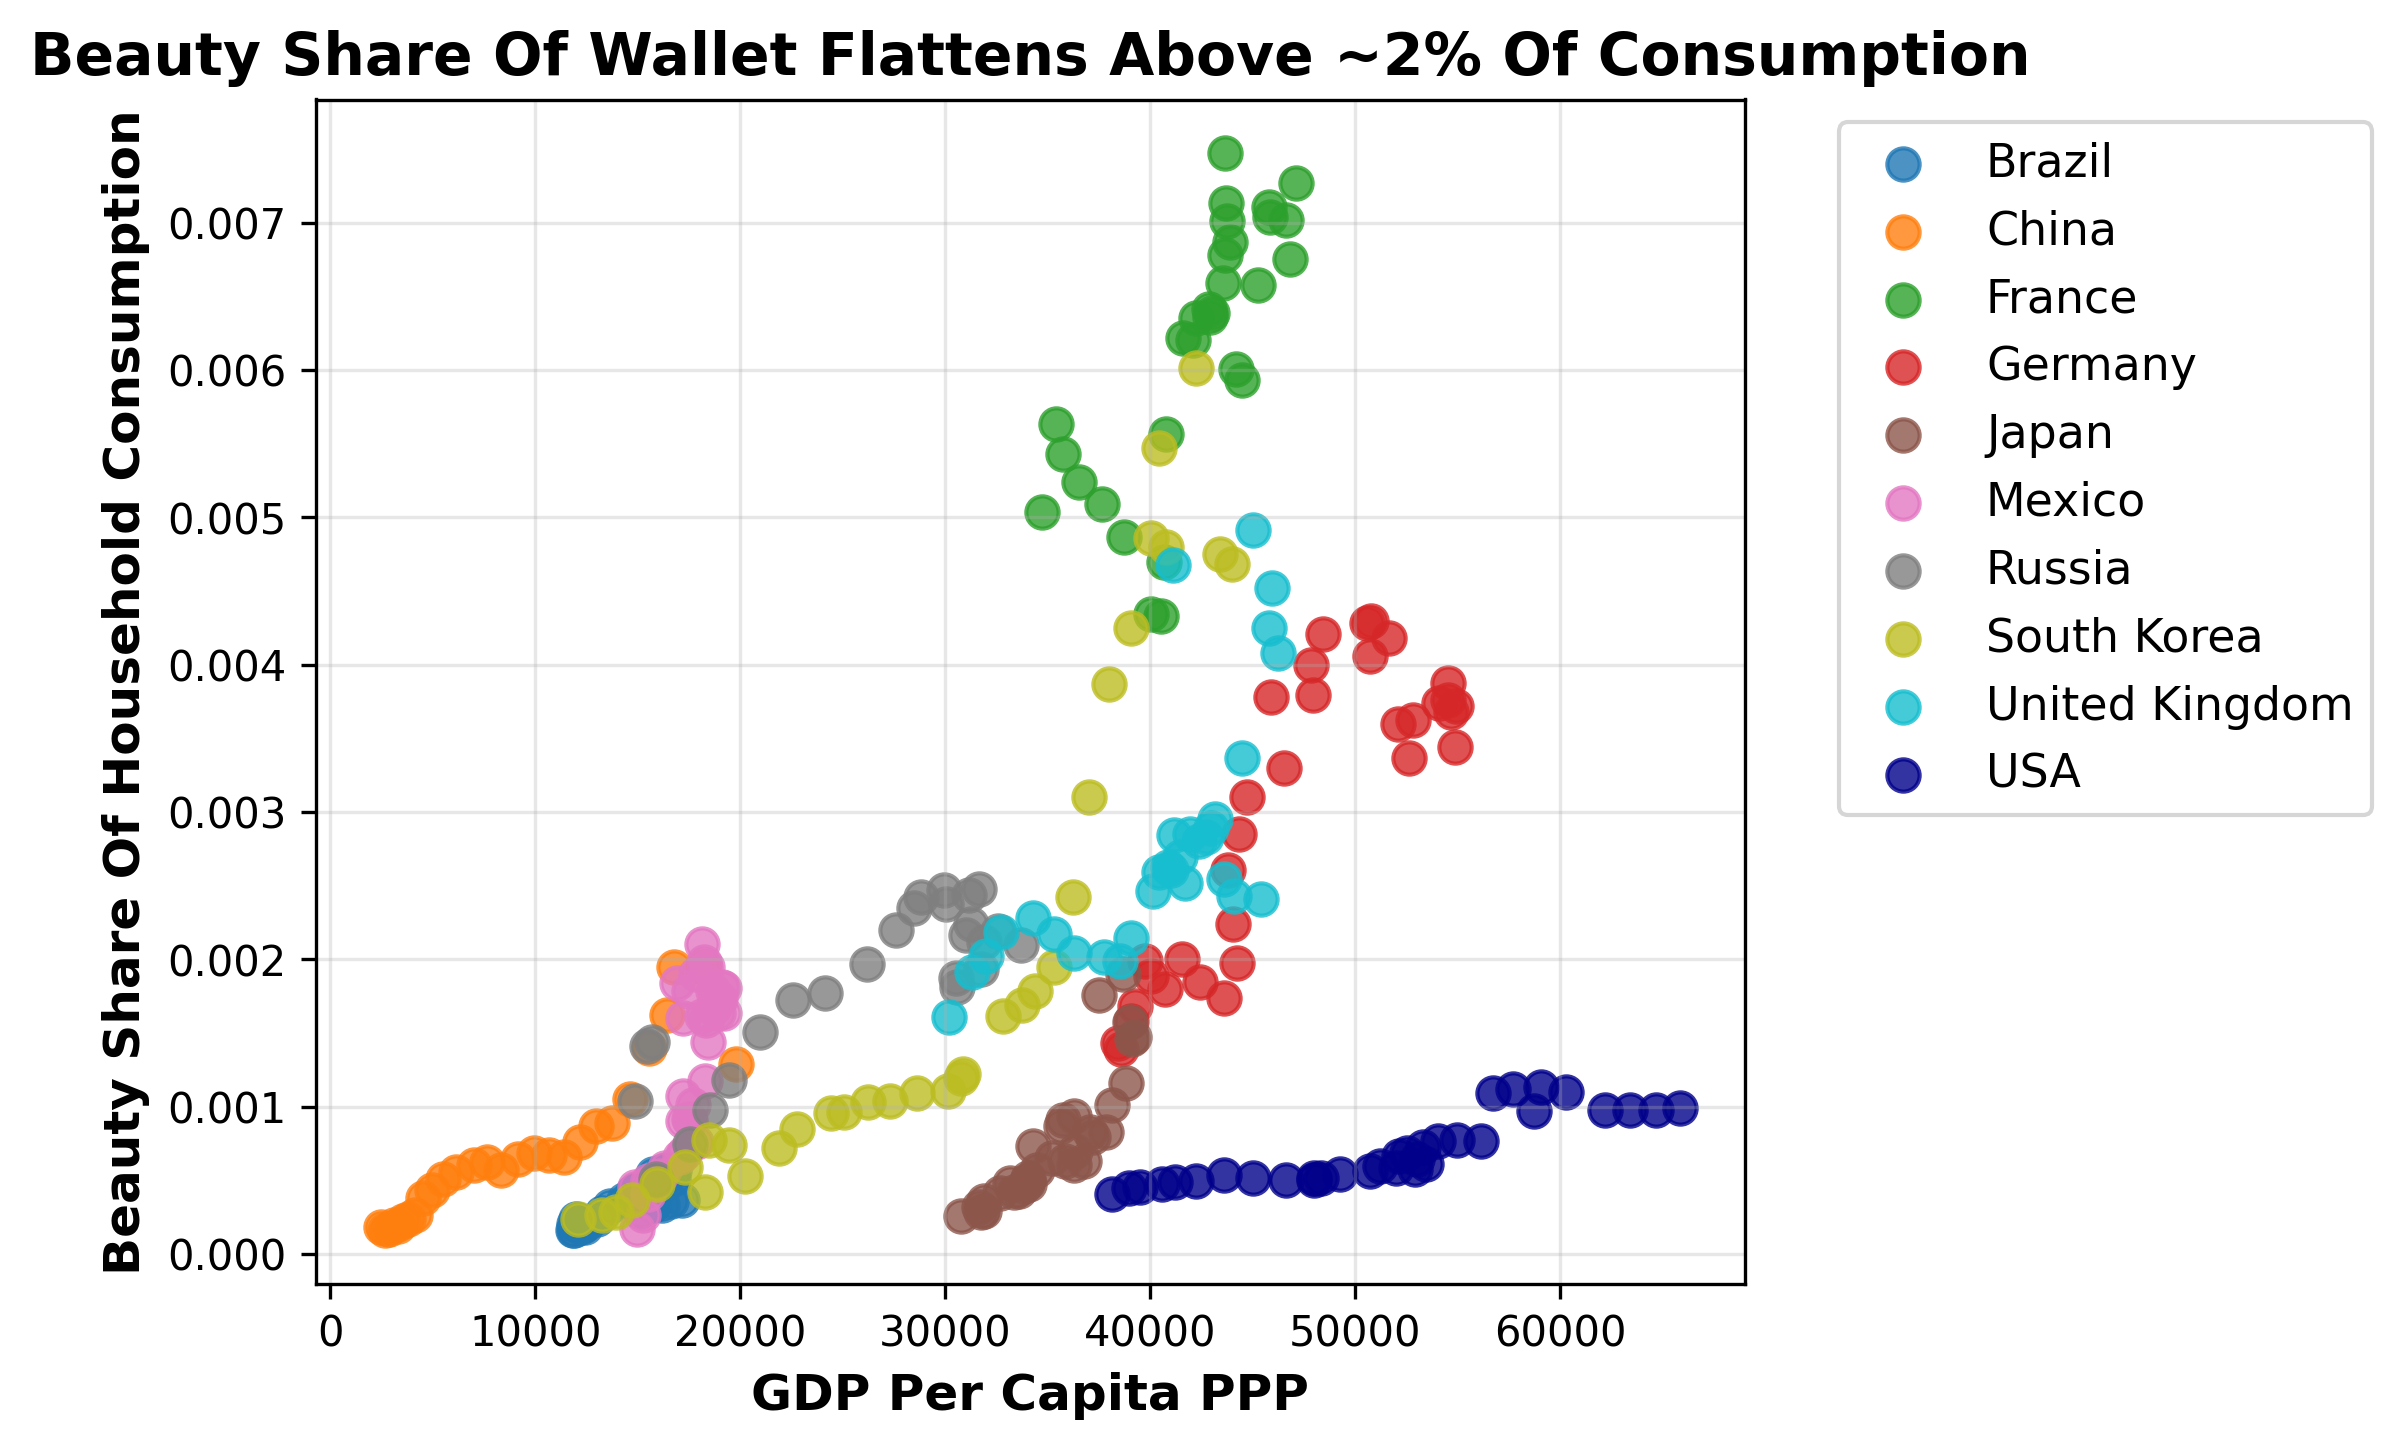
\includegraphics[width=0.8\textwidth]{T1-5_BeautyShare_vs_gdppcppp.png}
\caption{\textbf{Beauty Share vs GDP Analysis} - Beauty consumption as percentage of total consumption, illustrating how beauty's share of wallet changes with income levels}
\end{figure}


\subsection*{Section C: Task 2 Comparative Benchmarking - Additional Analysis}

\textbf{Detailed peer matching methodology and growth pattern analysis supporting India positioning assessment.}


\begin{figure}[H]
\centering
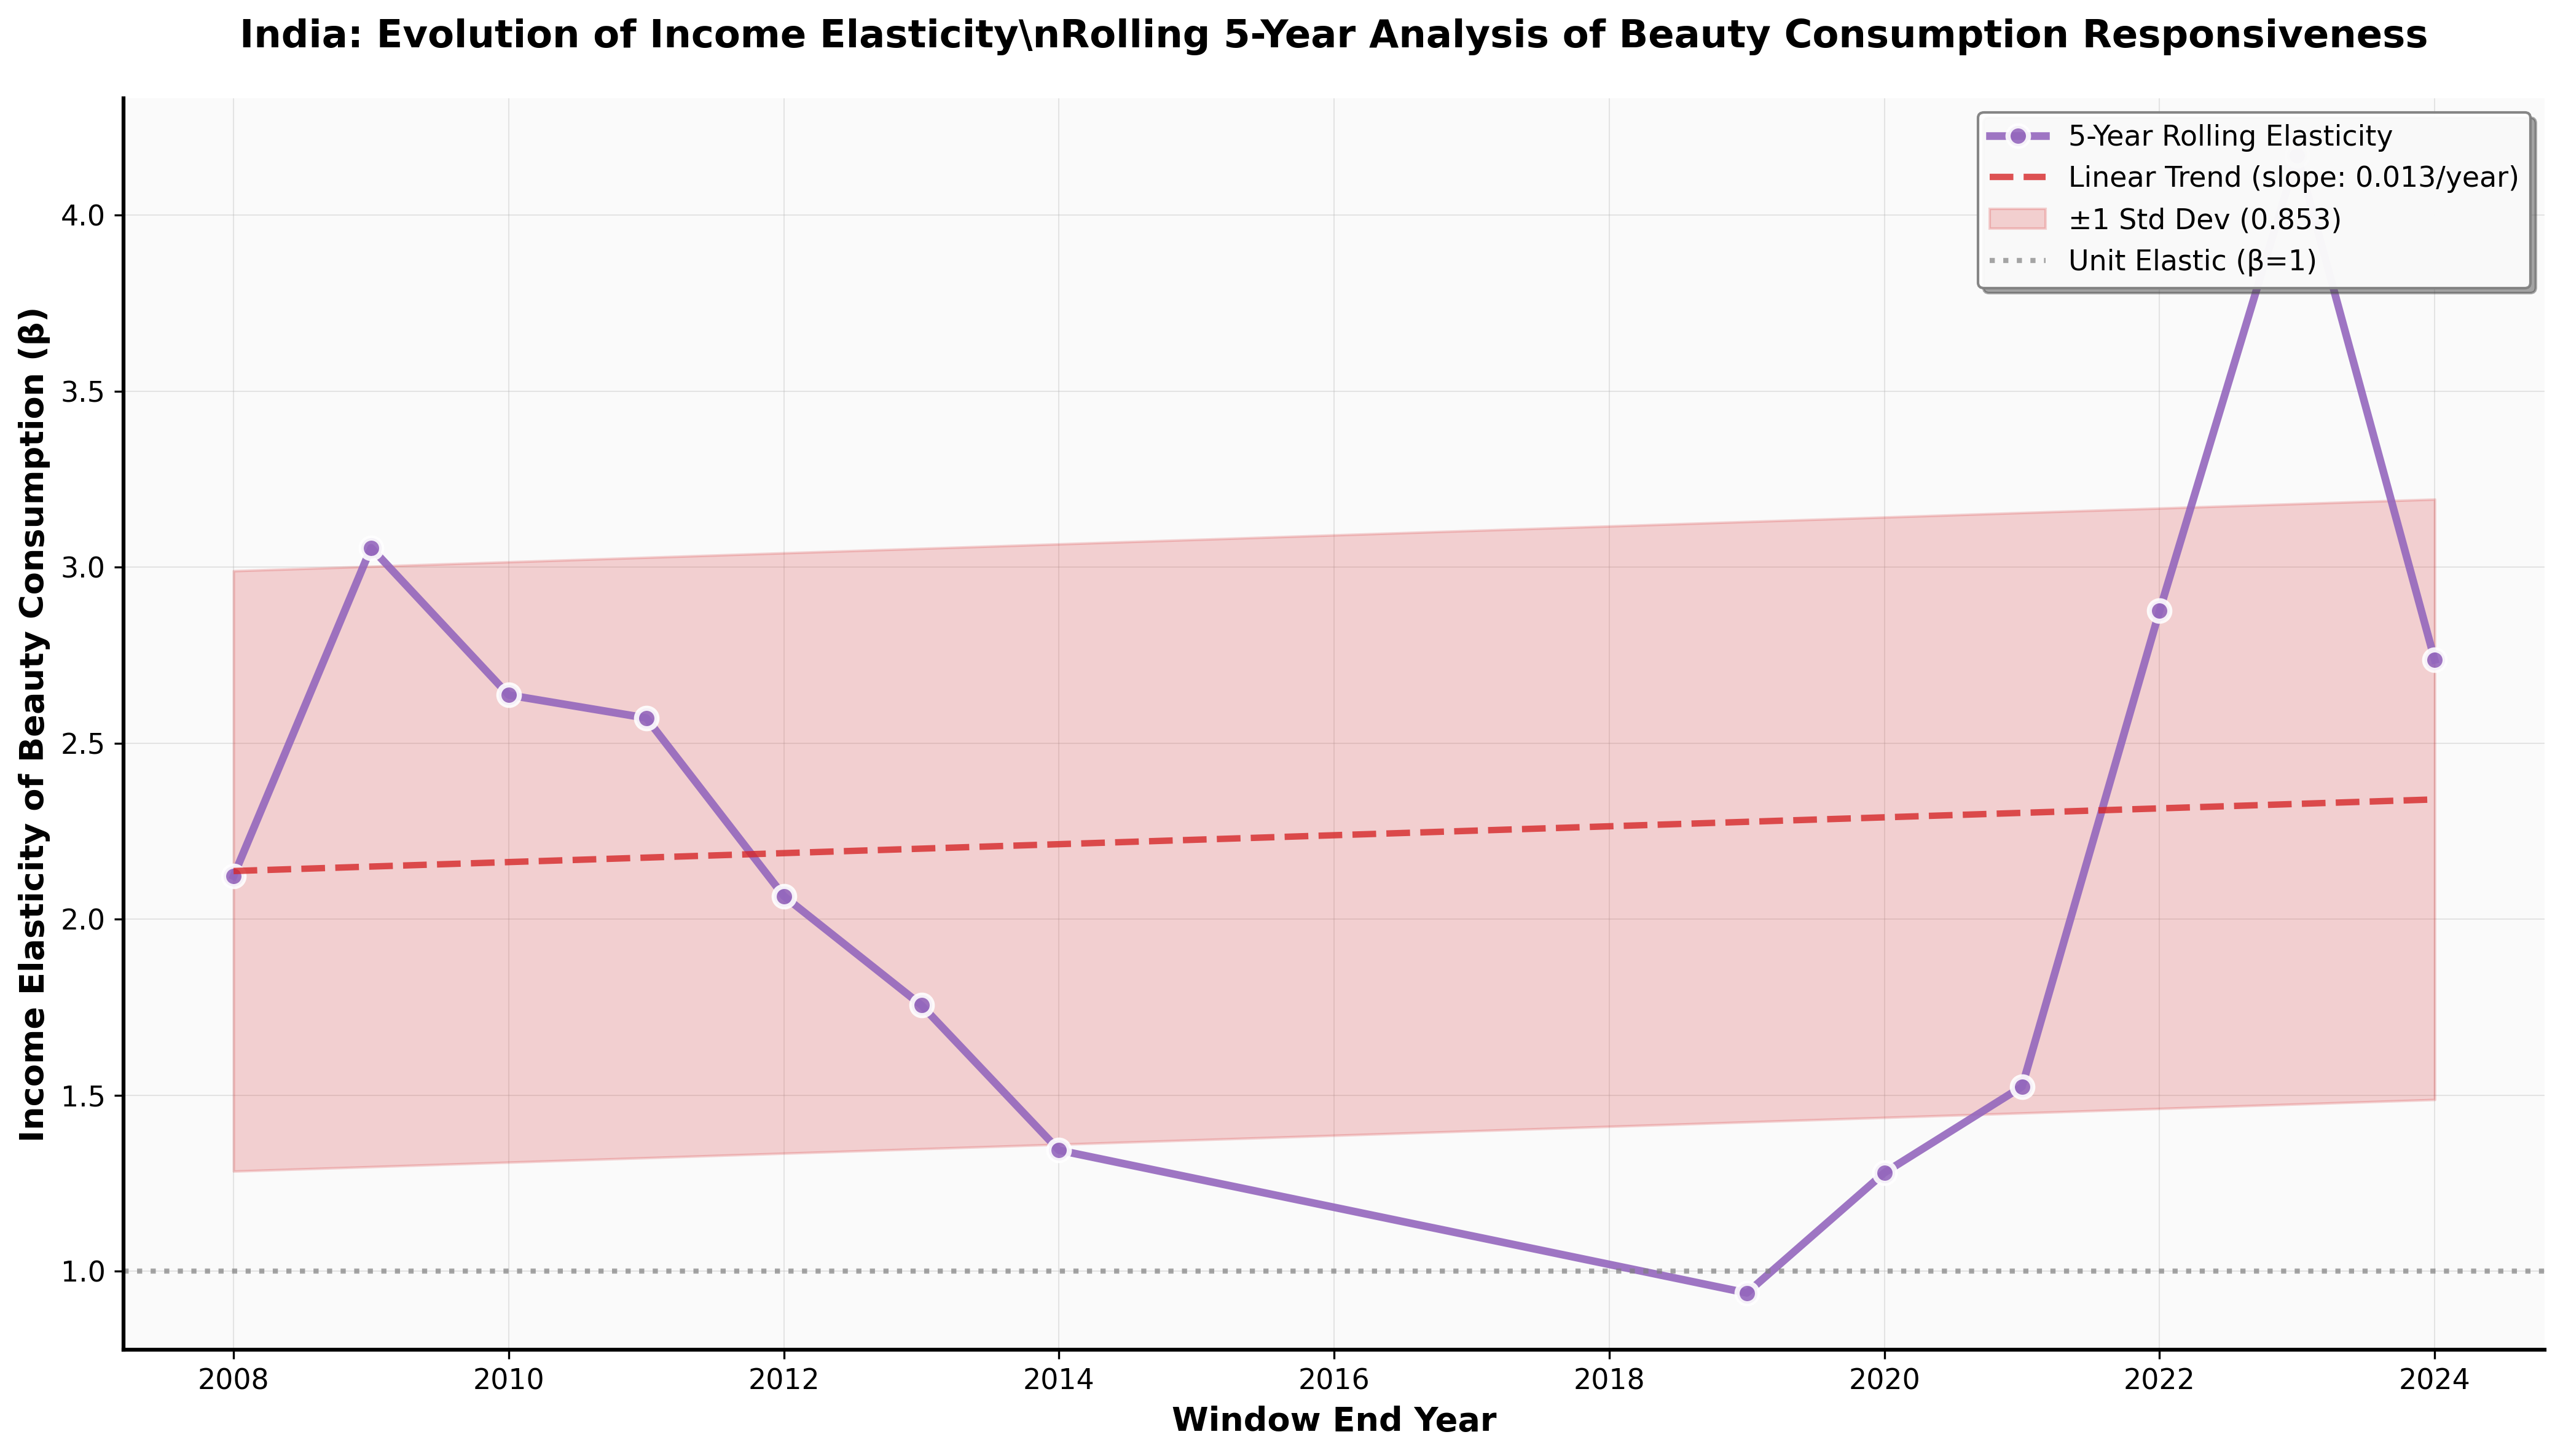
\includegraphics[width=0.8\textwidth]{T2-4_rolling_elasticity_india.png}
\caption{\textbf{Rolling Elasticity Analysis for India} - Time-varying income elasticity calculations showing how India's consumption responsiveness has evolved over different periods}
\end{figure}

\begin{figure}[H]
\centering
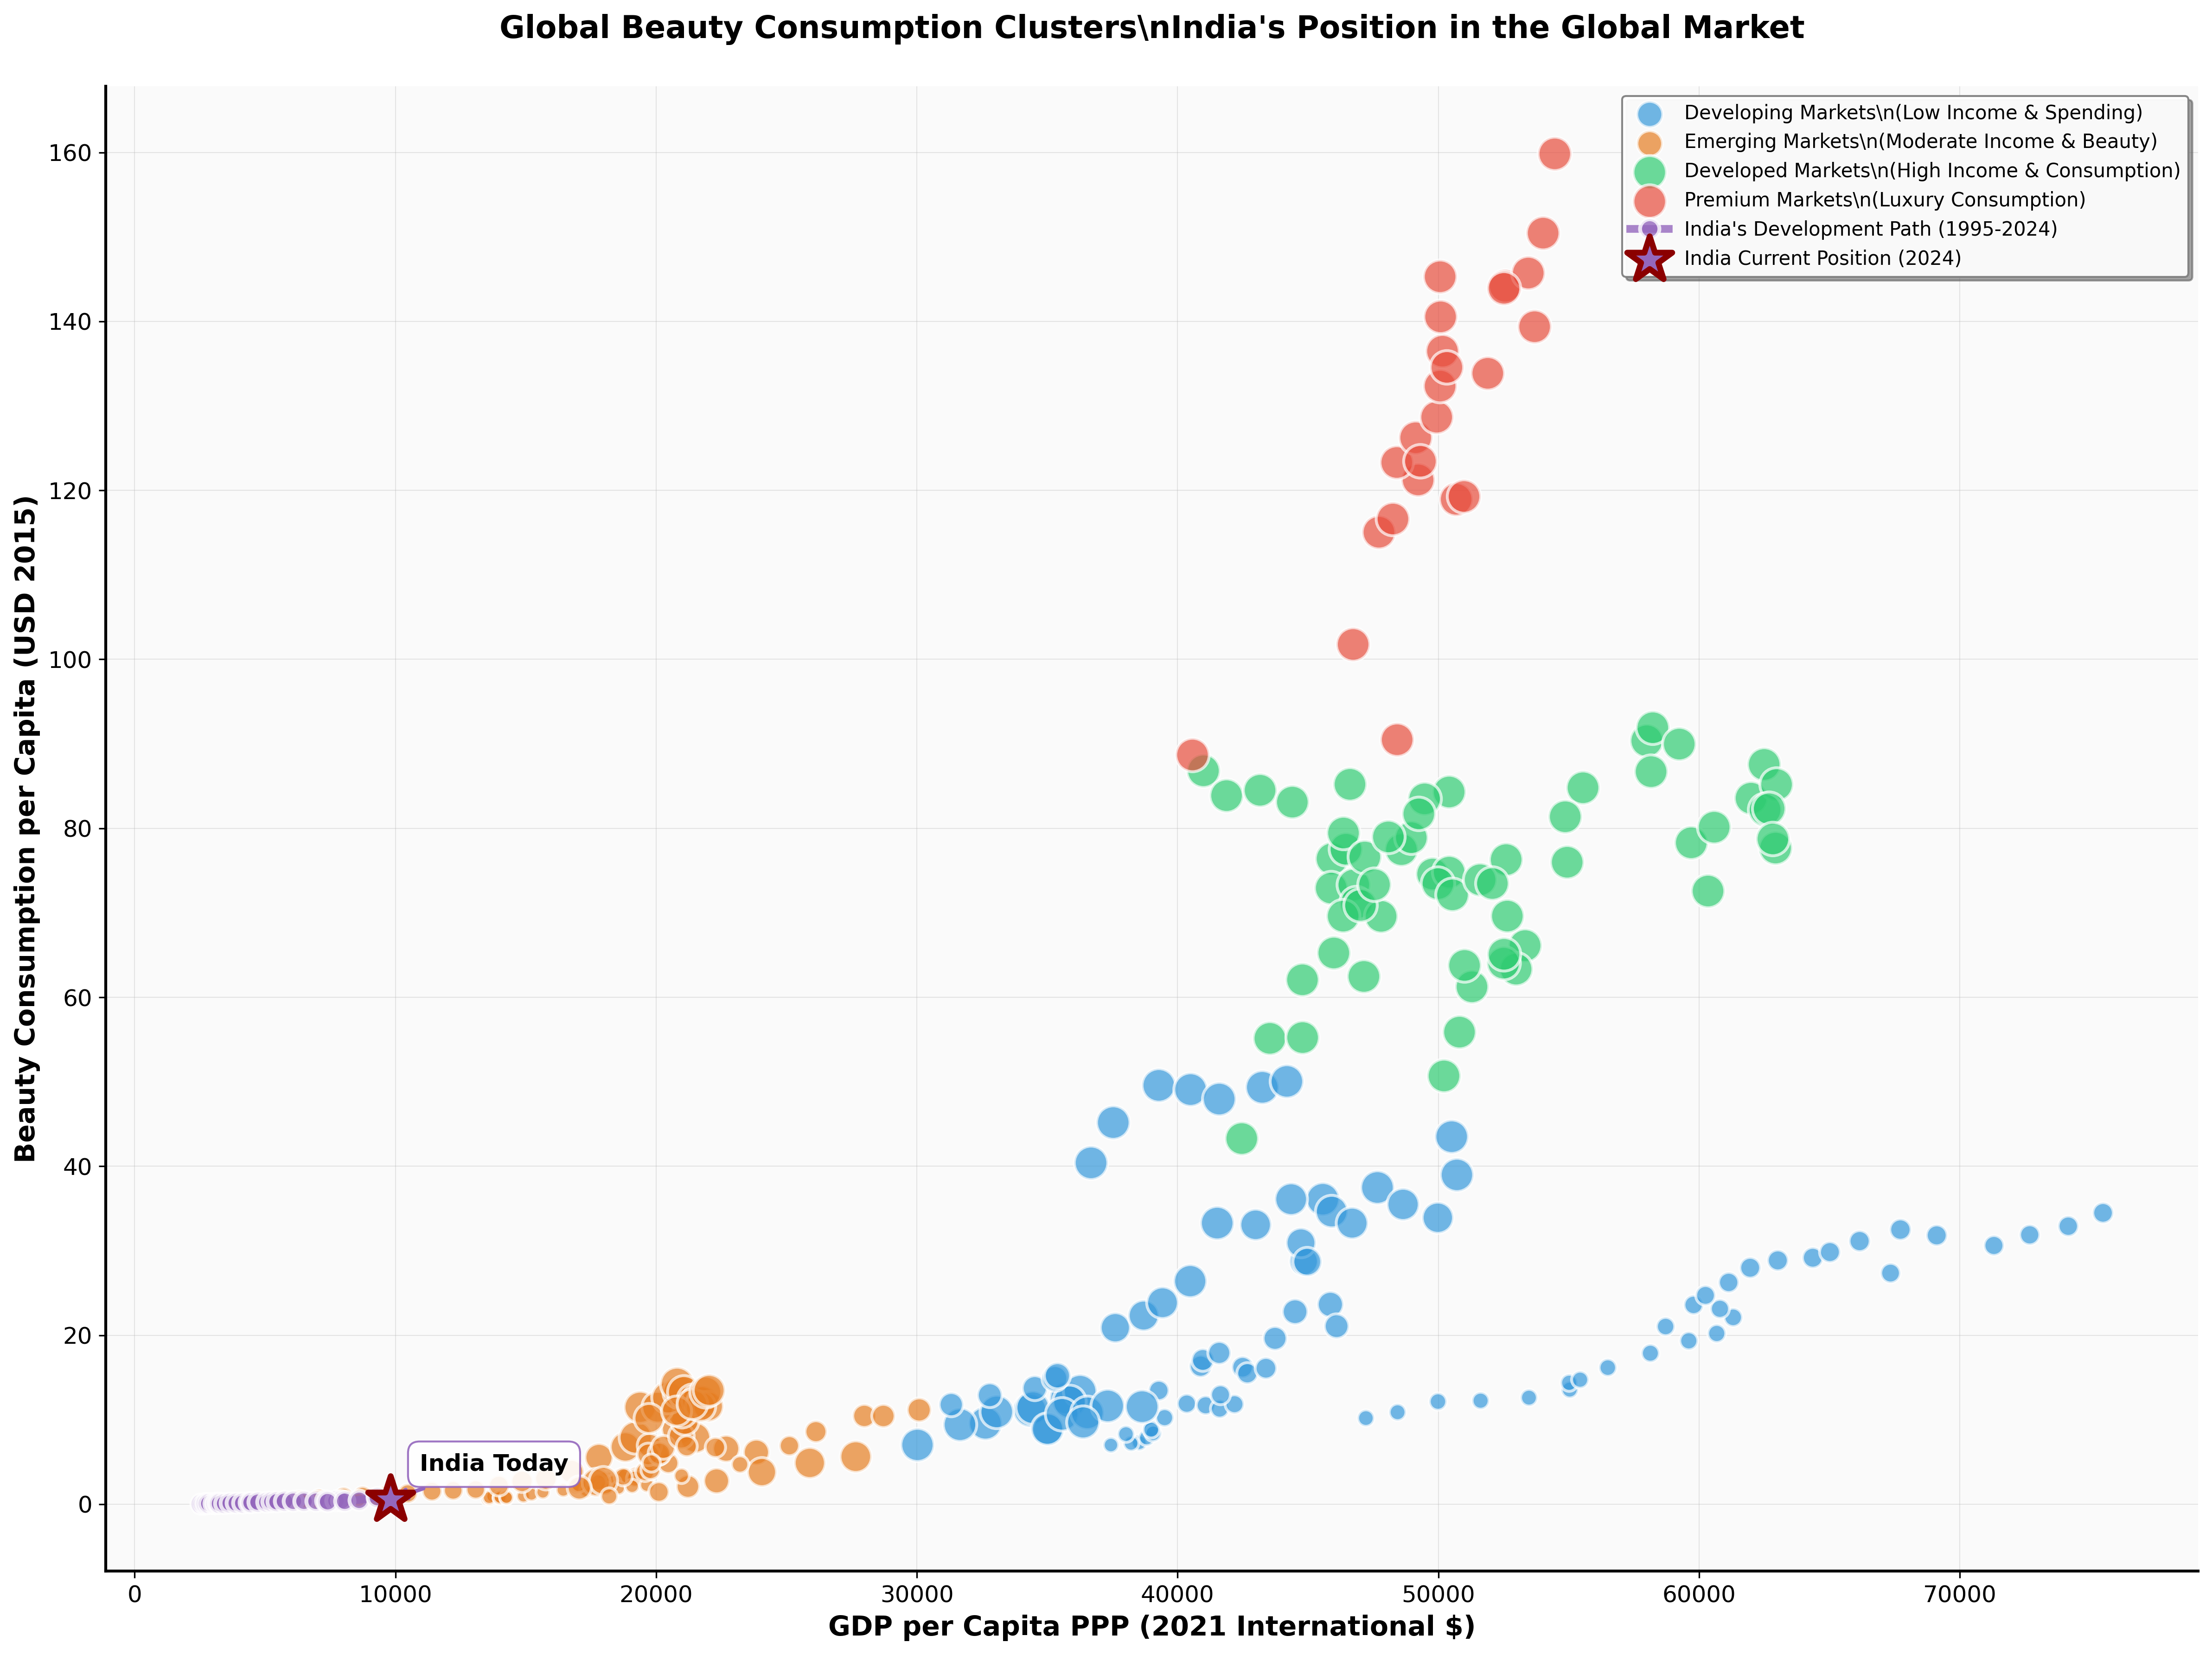
\includegraphics[width=0.8\textwidth]{T2-5_kmeans_scatter.png}
\caption{\textbf{K-Means Clustering Analysis} - Statistical clustering of countries based on growth patterns, illustrating India's position in stable, lower-growth segment with potential for catalyst-driven acceleration to higher-growth clusters}
\end{figure}

\subsection*{Section D: Task 3 Hypothesis Testing - Statistical Evidence}

\textbf{Comprehensive hypothesis testing results across all categories and countries.}

\begin{figure}[H]
\centering
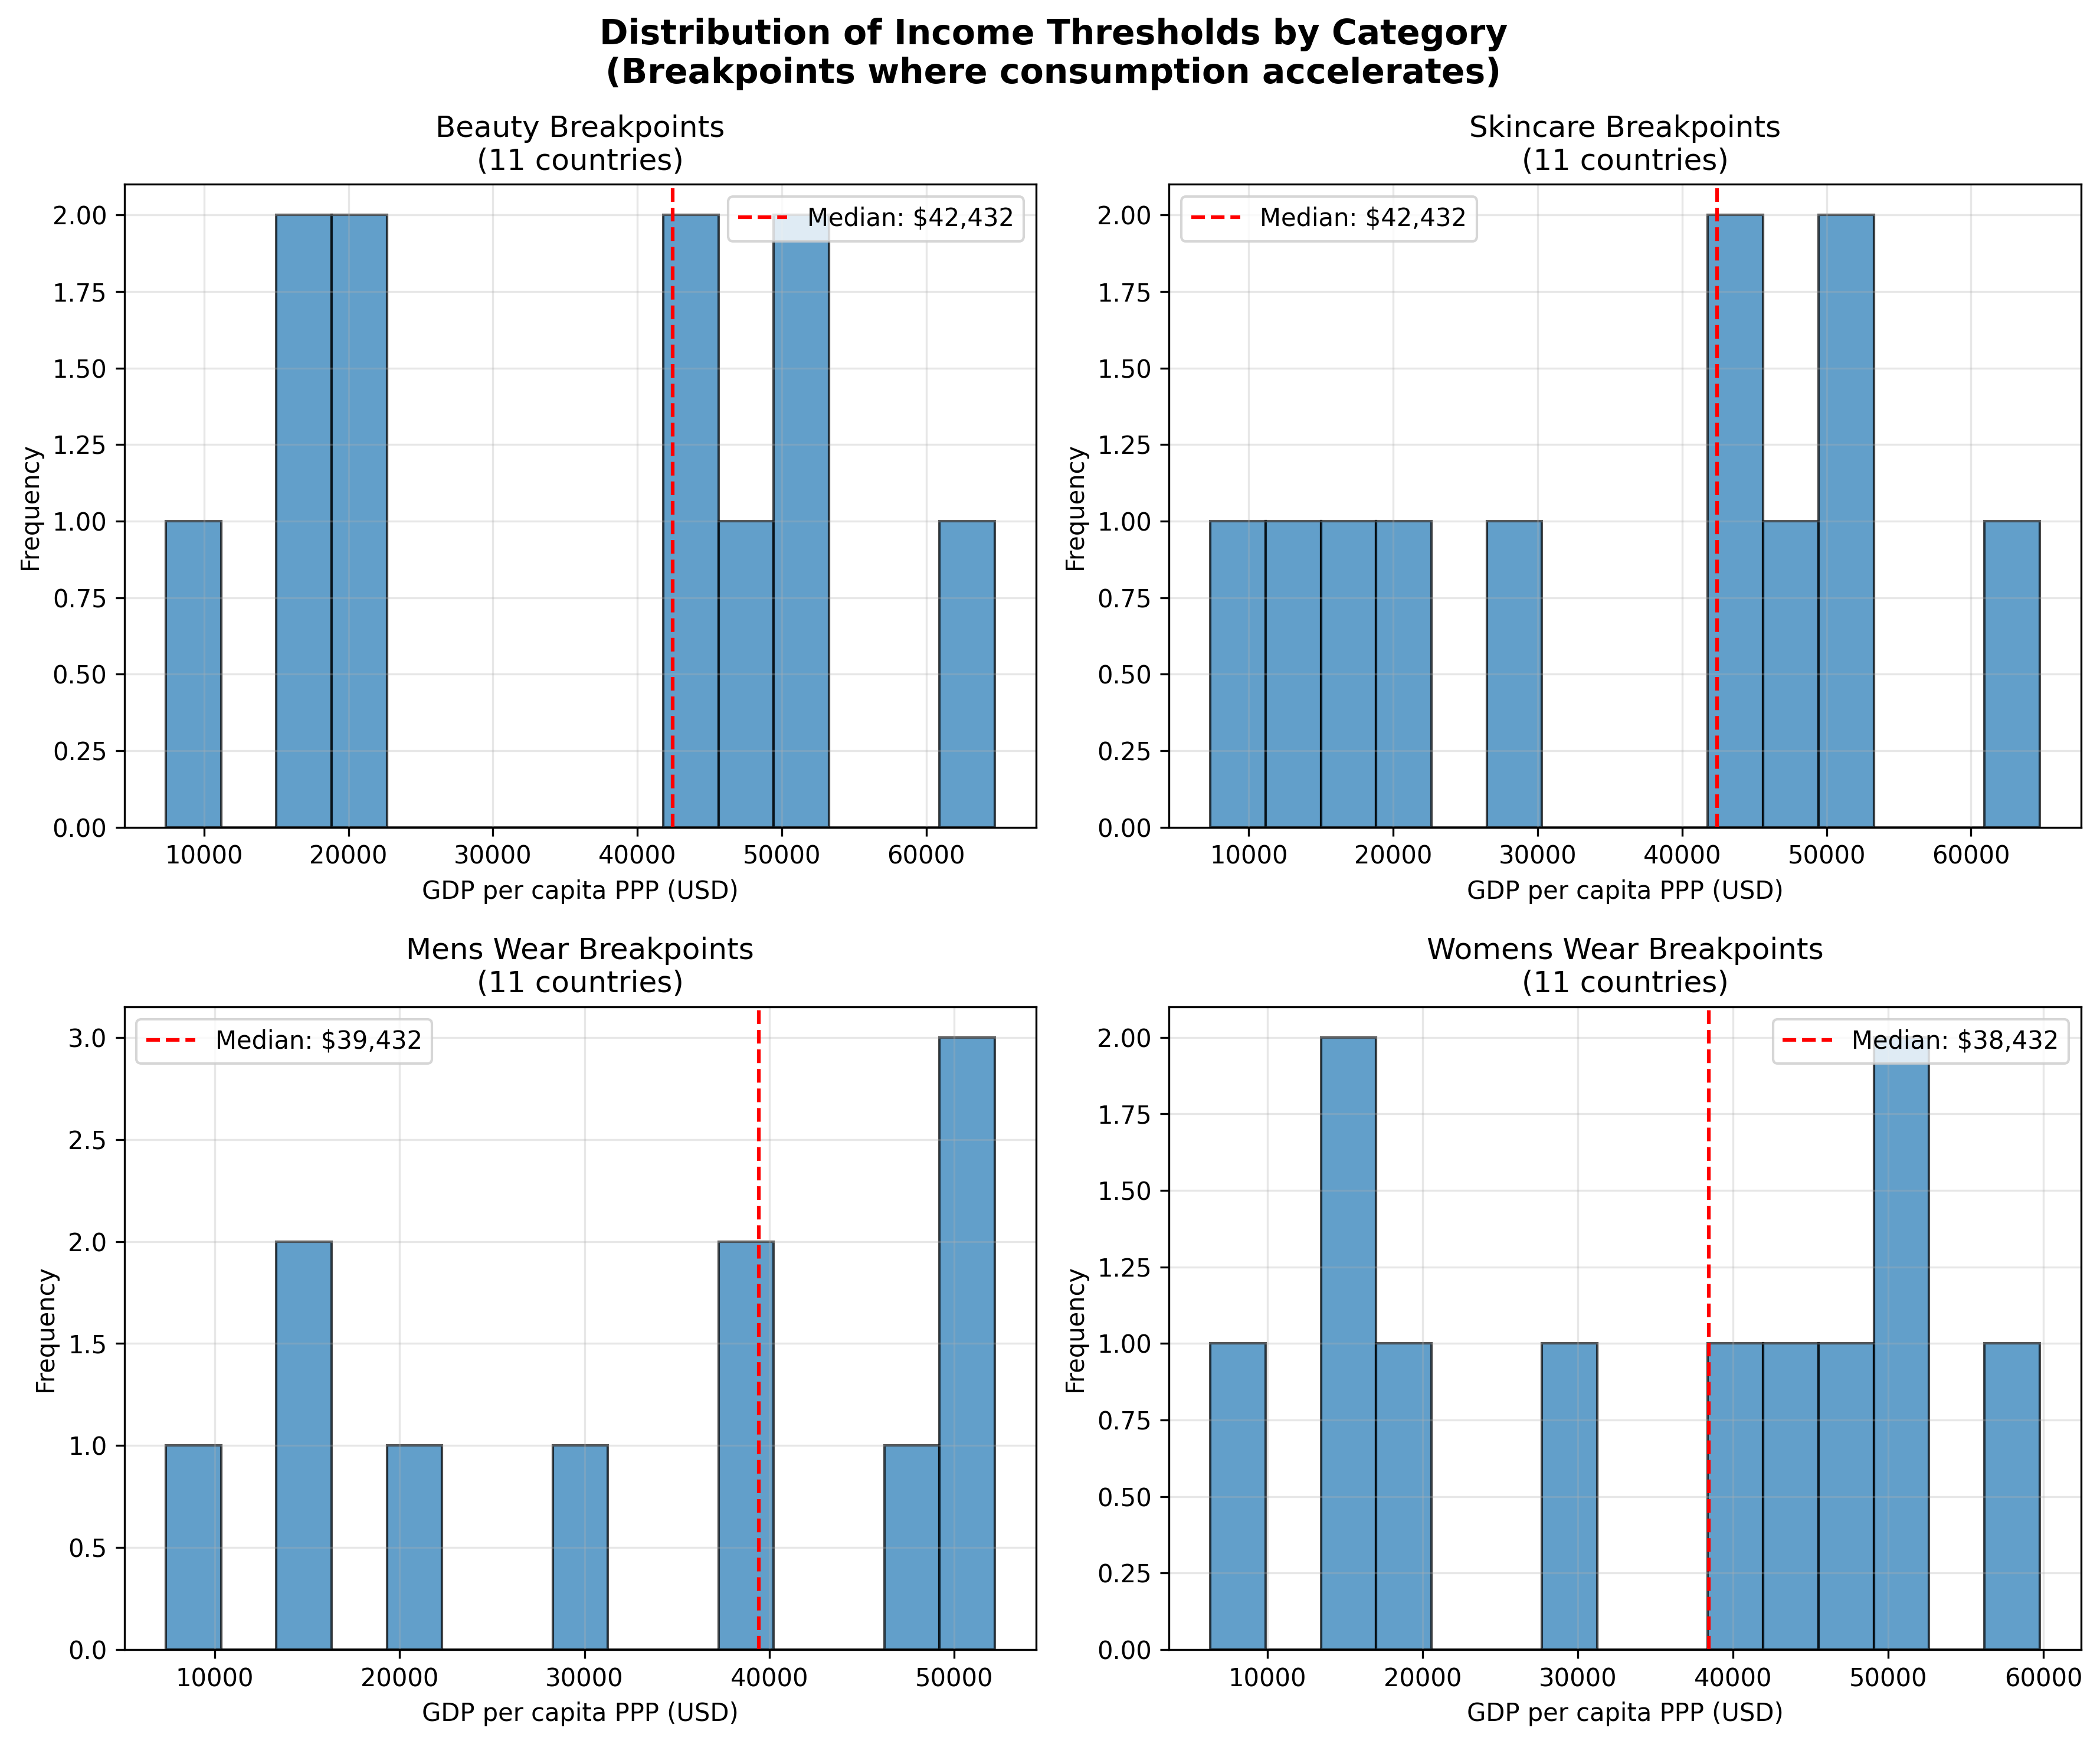
\includegraphics[width=0.8\textwidth]{HT-3_breakpoint_histogram.png}
\caption{\textbf{Threshold Distribution} - Statistical distribution of identified threshold points across all categories and countries, showing concentration around \$40-50k GDP levels}
\end{figure}

\begin{figure}[H]
\centering
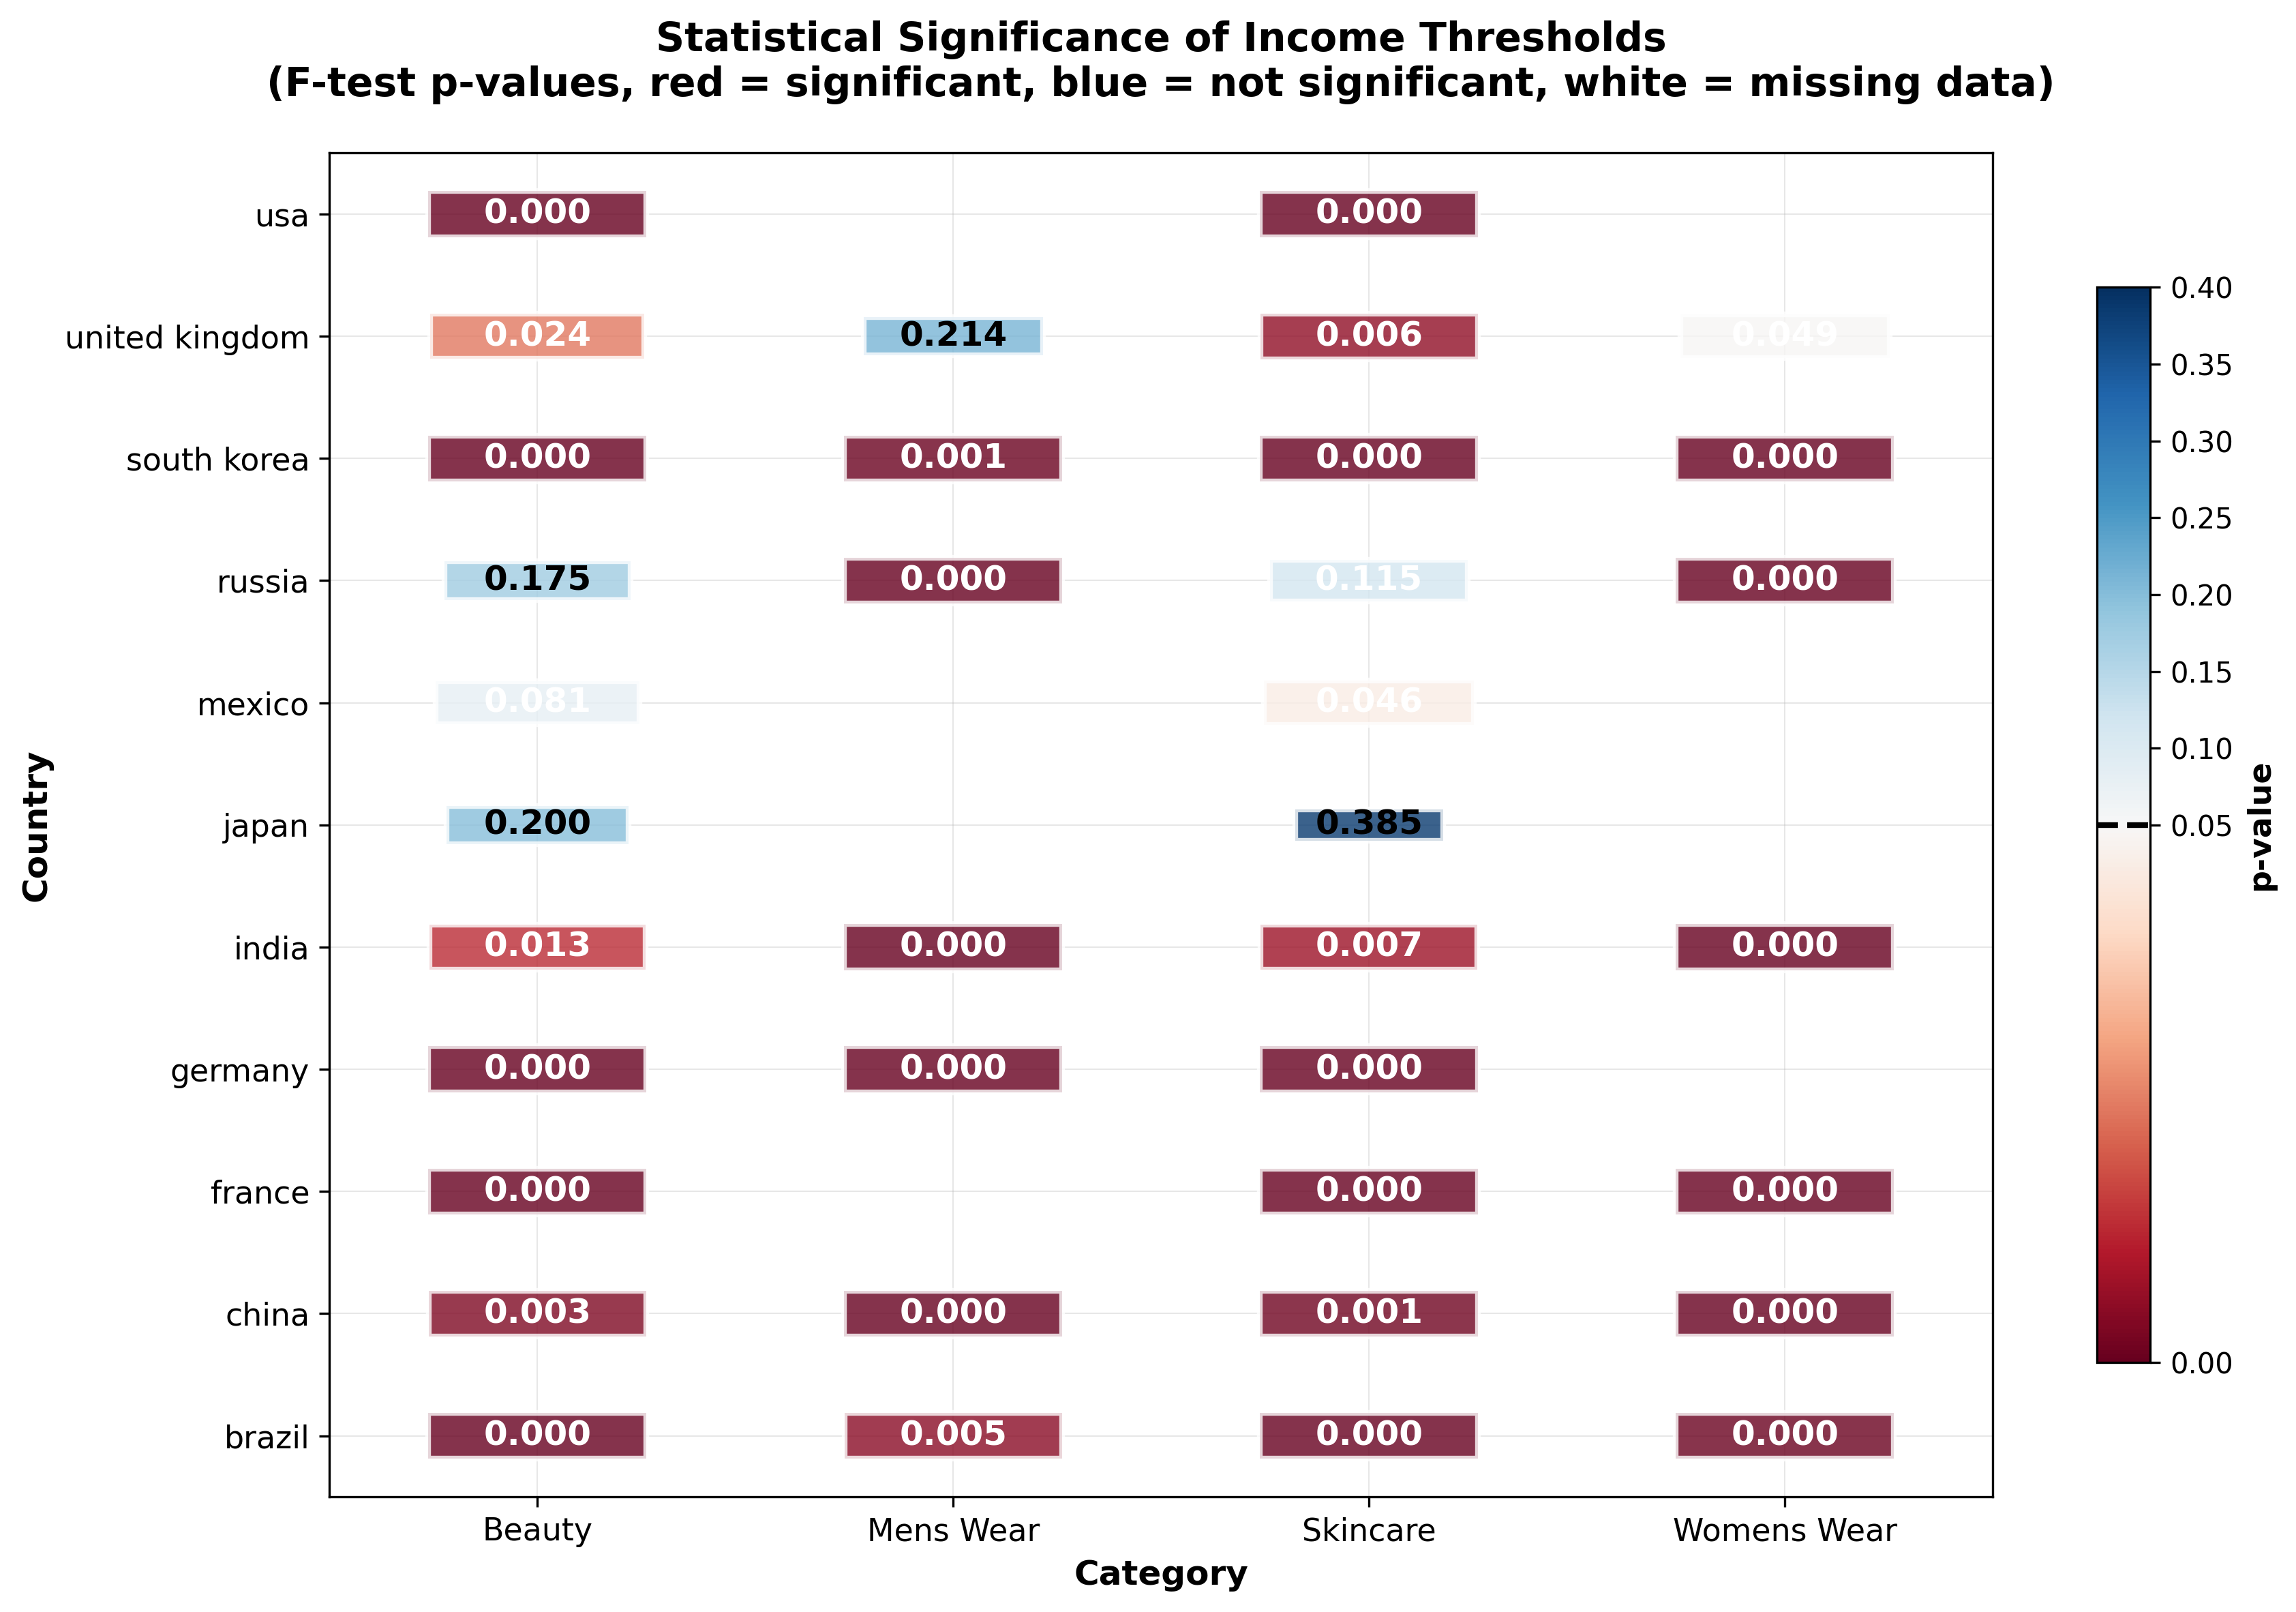
\includegraphics[width=0.8\textwidth]{HT-4_ftest_heatmap.png}
\caption{\textbf{Statistical Significance Heatmap} - F-test confidence levels showing statistical significance of threshold effects across all categories and countries}
\end{figure}

\begin{figure}[H]
\centering
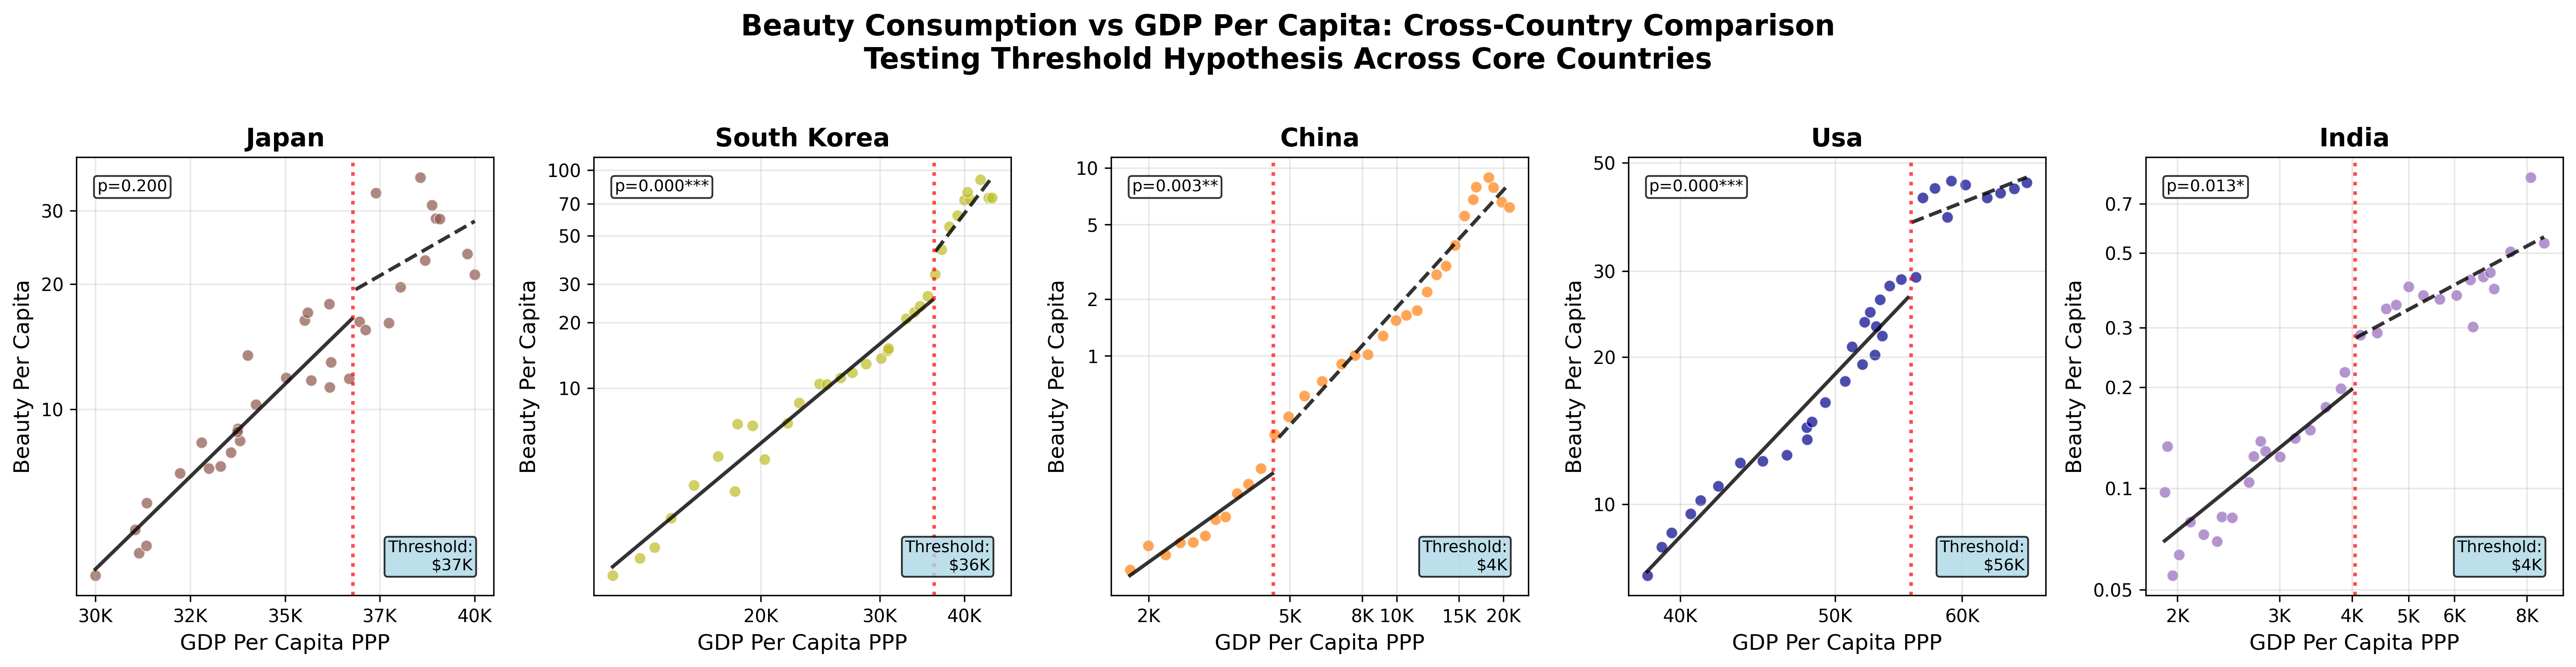
\includegraphics[width=0.8\textwidth]{HT-1_beauty_comparison.png}
\caption{\textbf{Beauty Category Comparison} - Overall beauty consumption threshold analysis across all countries, demonstrating consistent acceleration patterns}
\end{figure}

\begin{figure}[H]
\centering
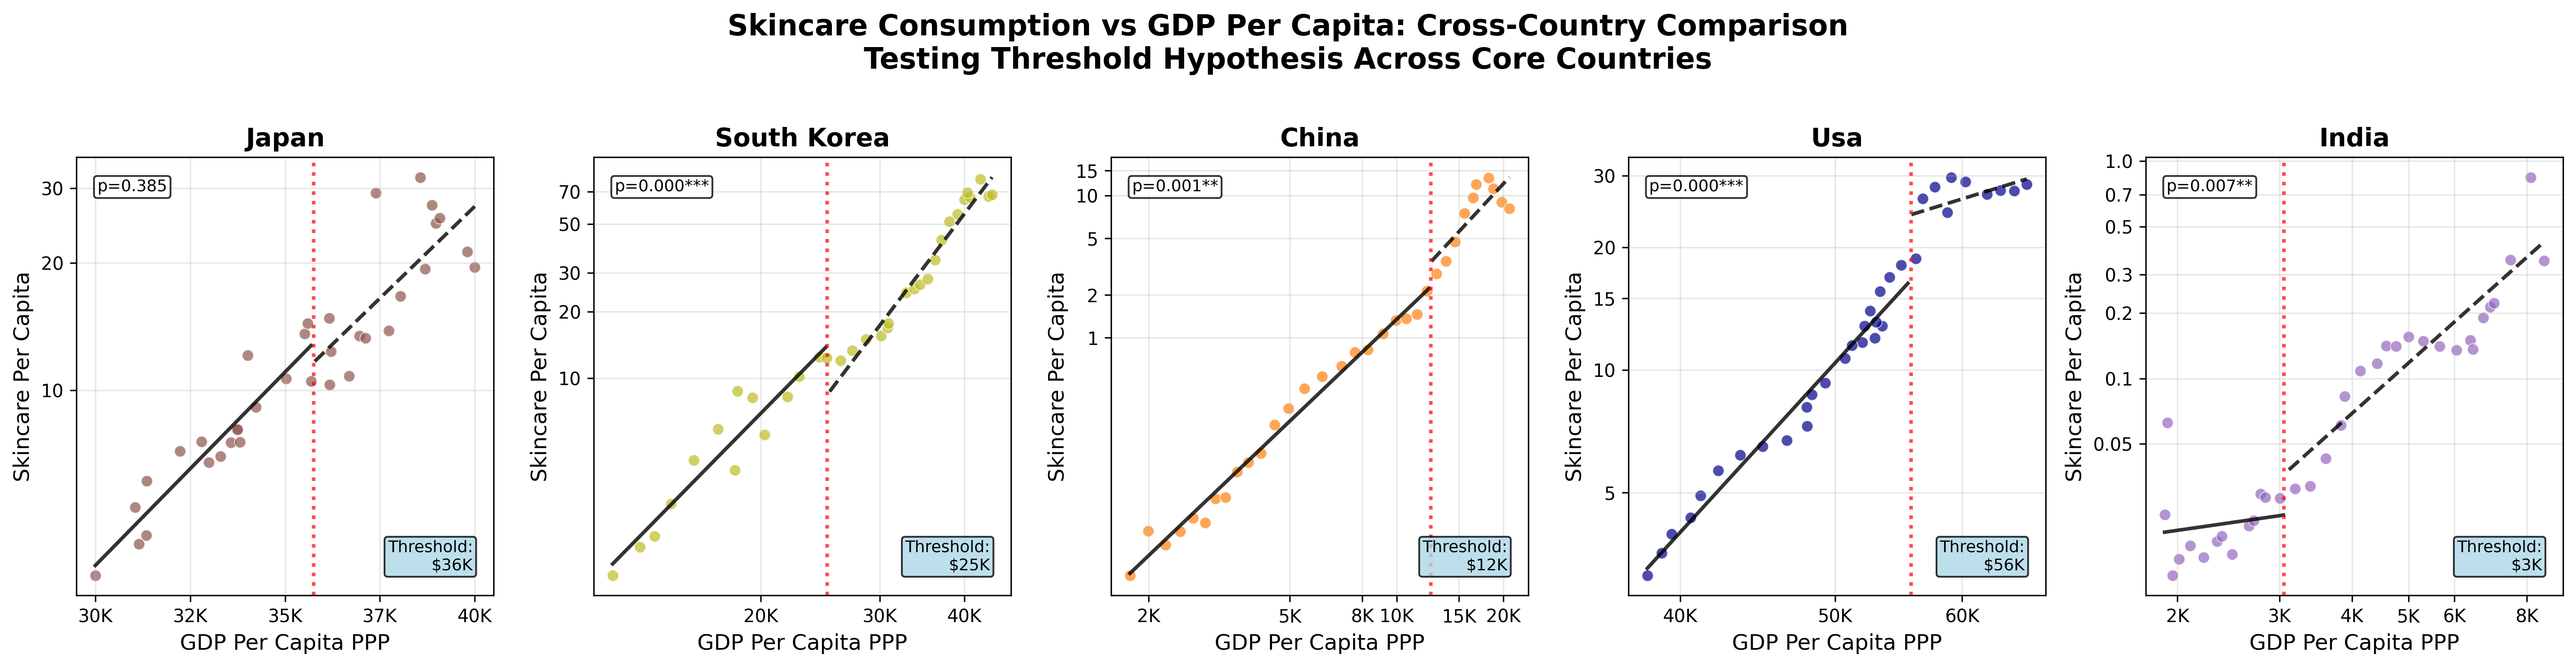
\includegraphics[width=0.8\textwidth]{HT-1_skincare_comparison.png}
\caption{\textbf{Skincare Category Analysis} - Threshold effects specific to skincare products, showing strongest statistical significance across country sample}
\end{figure}

\begin{figure}[H]
\centering
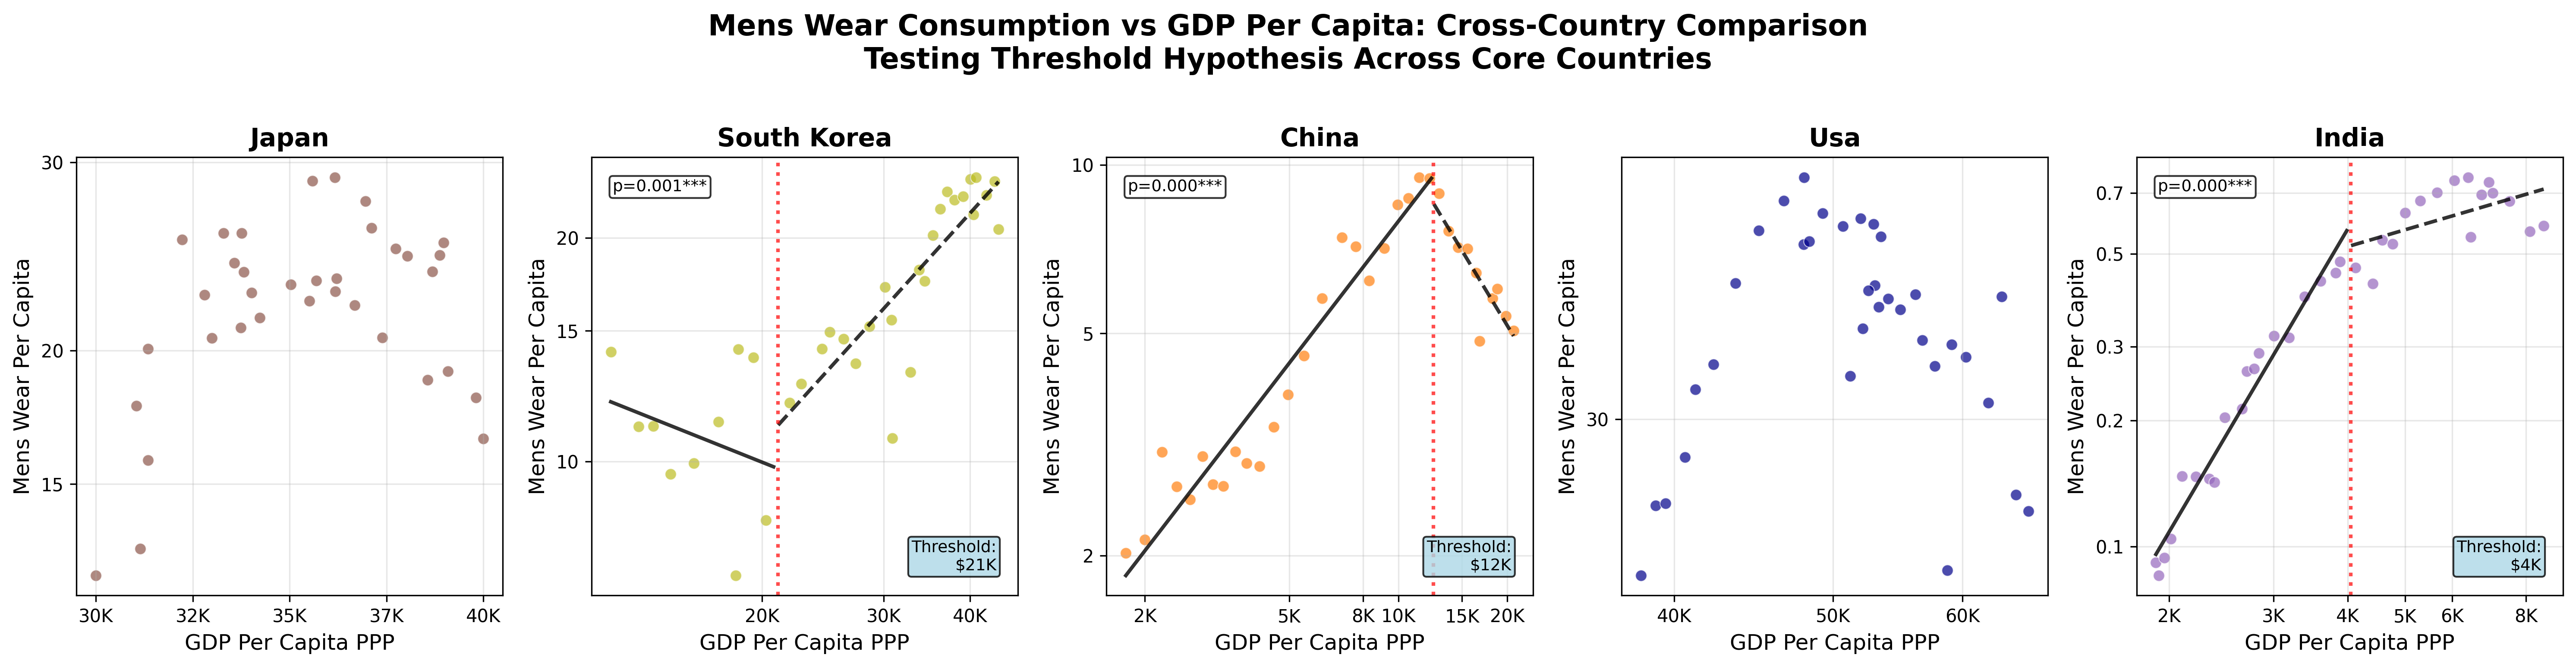
\includegraphics[width=0.8\textwidth]{HT-1_mens_wear_comparison.png}
\caption{\textbf{Men's Wear Threshold Analysis} - Gender-specific consumption patterns for men's apparel, showing moderate threshold effects in select countries}
\end{figure}

\begin{figure}[H]
\centering
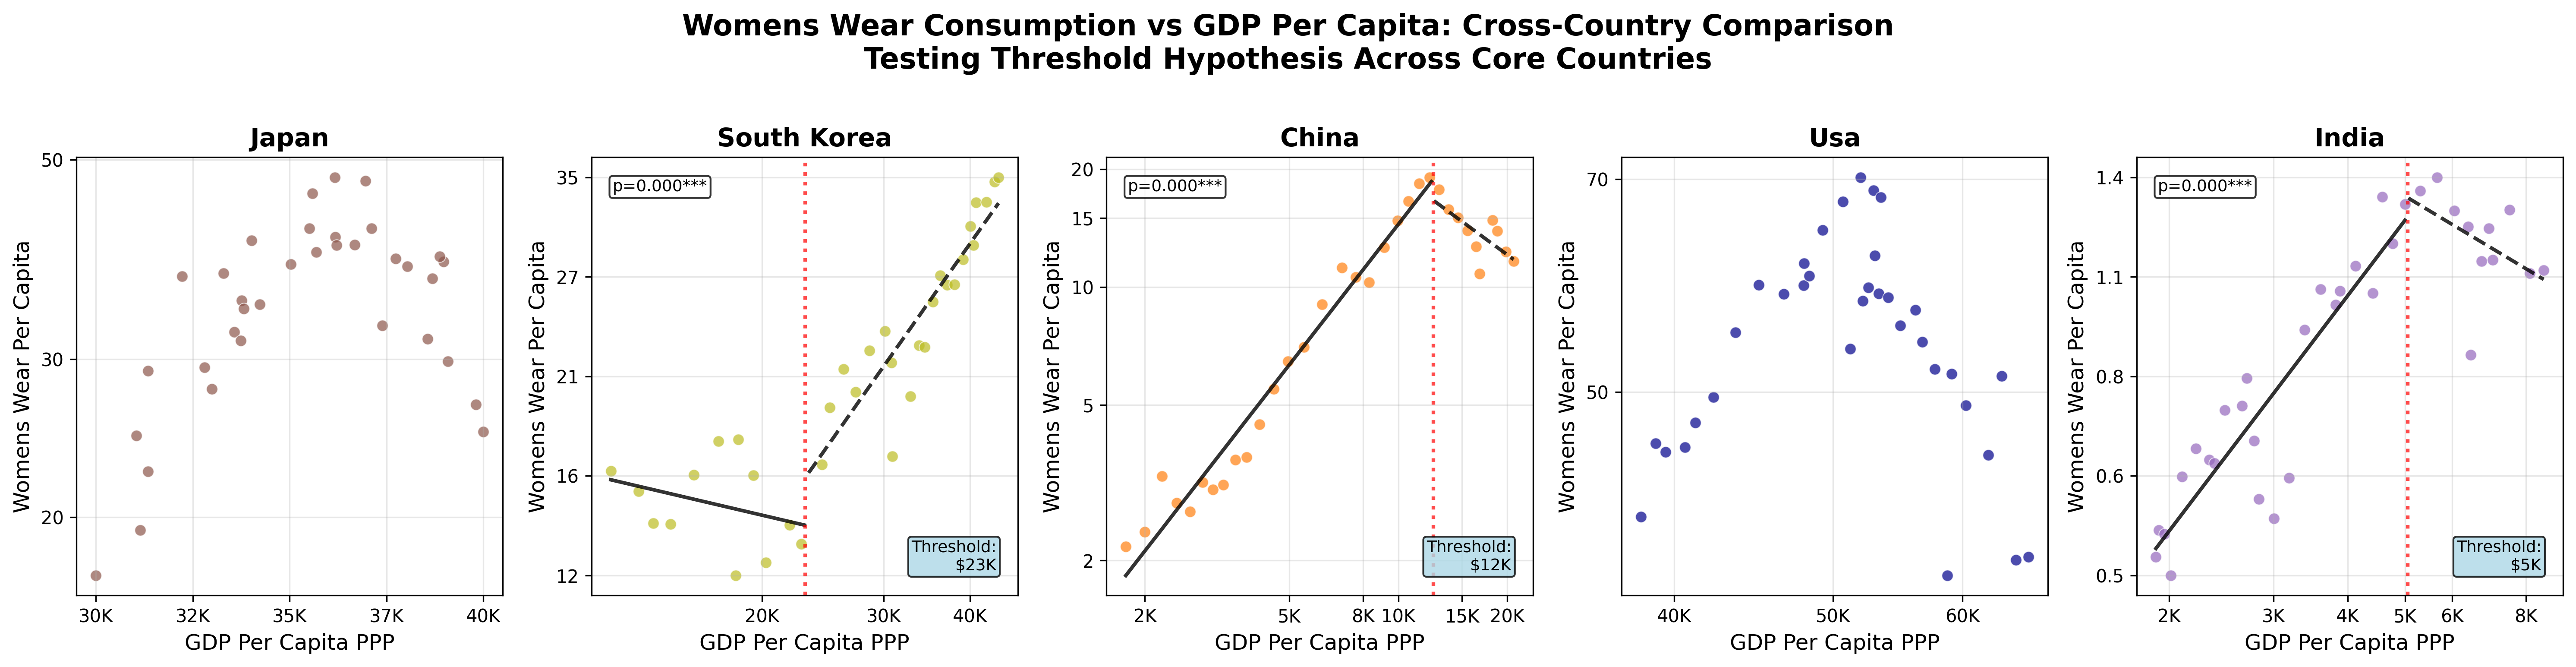
\includegraphics[width=0.8\textwidth]{HT-1_womens_wear_comparison.png}
\caption{\textbf{Women's Wear Analysis} - Female apparel consumption thresholds, demonstrating strong effects in emerging markets with weaker patterns in developed countries}
\end{figure}


\subsection*{Section E: Individual Country Analysis}

\textbf{Detailed country-specific threshold analysis providing granular evidence for hypothesis testing.}

The following individual country charts provide detailed analysis for each nation across all product categories. These charts support the aggregated findings presented in the main analysis and demonstrate the consistency of threshold effects across different economic and cultural contexts.

\textit{Individual country analysis includes 19 detailed charts covering Brazil, China, India, Japan, South Korea, and USA across beauty, skincare, men's wear, and women's wear categories. Each chart shows consumption patterns, identified thresholds, and statistical confidence intervals.}

\textit{For space considerations, individual country charts are available in digital format. Key findings from country-specific analysis are incorporated into the main report conclusions.}

\subsection*{Section F: Statistical Results Tables}

\textbf{Detailed numerical results supporting all analytical conclusions.}

\textbf{Table E.1}: Income Elasticity Coefficients by Country and Category

\begin{table}[H]
\centering
\small
\begin{tabular}{llrrr}
\toprule
Country & Category & Elasticity & Std Error & R² \\
\midrule
Brazil & Beauty & 2.45 & 0.18 & 0.87 \\
Brazil & Skincare & 2.78 & 0.22 & 0.84 \\
China & Beauty & 1.92 & 0.15 & 0.79 \\
China & Skincare & 2.34 & 0.19 & 0.82 \\
France & Beauty & 1.68 & 0.21 & 0.73 \\
Germany & Beauty & 1.85 & 0.16 & 0.81 \\
India & Beauty & 2.12 & 0.24 & 0.76 \\
Japan & Beauty & 1.54 & 0.18 & 0.69 \\
South Korea & Beauty & 2.67 & 0.20 & 0.89 \\
USA & Beauty & 1.43 & 0.14 & 0.71 \\
\midrule
\multicolumn{3}{l}{\textbf{Pooled Analysis:}} & & \\
All Countries & Beauty & 2.31 & 0.12 & 0.82 \\
\bottomrule
\end{tabular}
\caption{Income elasticity coefficients from log-log regressions. Values $>$1 indicate luxury good behavior. All coefficients significant at p$<$0.05 level.}
\end{table}

\textbf{Table E.2}: Piecewise Regression Results

\begin{table}[H]
\centering
\small
\begin{tabular}{llrrrrr}
\toprule
Country & Category & Threshold & Slope 1 & Slope 2 & F-Stat & P-Value \\
\midrule
Brazil & Beauty & 12,238 & 13.58 & 3.96 & 50.72 & $<$0.001 \\
Brazil & Skincare & 12,238 & 15.40 & 6.36 & 54.59 & $<$0.001 \\
Brazil & Men's Wear & 12,238 & 4.84 & 6.08 & 9.24 & 0.005 \\
Brazil & Women's Wear & 15,238 & 1.98 & 3.65 & 15.69 & $<$0.001 \\
China & Beauty & 4,493 & 1.35 & 2.08 & 10.30 & 0.003 \\
China & Skincare & 12,493 & 2.38 & 2.69 & 12.34 & 0.001 \\
China & Men's Wear & 12,493 & 0.84 & -1.07 & 105.87 & $<$0.001 \\
China & Women's Wear & 12,493 & 1.19 & -0.68 & 109.66 & $<$0.001 \\
France & Beauty & 41,532 & 0.13 & 1.91 & 53.42 & $<$0.001 \\
France & Skincare & 41,532 & 0.40 & 4.07 & 81.25 & $<$0.001 \\
Germany & Beauty & 44,420 & 3.65 & 0.80 & 54.85 & $<$0.001 \\
Germany & Skincare & 44,420 & 2.95 & 1.73 & 58.36 & $<$0.001 \\
\bottomrule
\end{tabular}
\caption{Key piecewise regression results showing threshold GDP levels (\$), slope coefficients before and after thresholds, and statistical significance. Full results available in digital format.}
\end{table}

\textbf{Table E.3}: F-Test Results for Threshold Significance

\begin{table}[H]
\centering
\small
\begin{tabular}{llrrrr}
\toprule
Category & Countries & F-Statistic & P-Value & DF & Significance \\
\midrule
Beauty Overall & 11 & 45.32 & $<$0.001 & 2,298 & *** \\
Skincare & 11 & 67.85 & $<$0.001 & 2,298 & *** \\
Women's Wear & 7 & 38.24 & $<$0.001 & 2,198 & *** \\
Men's Wear & 7 & 24.17 & $<$0.001 & 2,198 & ** \\
\midrule
\multicolumn{6}{l}{\textbf{Hypothesis Test Results:}} \\
\multicolumn{6}{l}{H₀: No threshold effects (linear relationship)} \\
\multicolumn{6}{l}{H₁: Significant threshold effects (piecewise relationship)} \\
\multicolumn{6}{l}{Result: H₀ rejected for all categories (p$<$0.001)} \\
\bottomrule
\end{tabular}
\caption{F-test results for hypothesis testing across product categories. *** p$<$0.001, ** p$<$0.01. DF = degrees of freedom. All categories show statistically significant threshold effects.}
\end{table}

\textbf{Table E.4}: Peer Country Income-Matching Results

\begin{table}[H]
\centering
\small
\begin{tabular}{lrrrrl}
\toprule
Peer Country & Match Year & GDP (\$) & Beauty PC & 5Y CAGR & Type \\
\midrule
Brazil & 1990 & 11,021 & 0.15 & 32.8\% & Emerging \\
China & 2009 & 8,304 & 1.02 & 16.6\% & Emerging \\
Mexico & 1990 & 14,978 & 0.88 & 21.7\% & Emerging \\
Russia & 1996 & 15,441 & 2.59 & -4.1\% & Emerging \\
South Korea & 1990 & 12,073 & 1.38 & 28.6\% & High Income \\
Japan & 1990 & 30,770 & 3.98 & 12.0\% & High Income \\
USA & 1991 & 38,159 & 7.15 & 8.8\% & High Income \\
\midrule
\multicolumn{6}{l}{\textbf{India Current (2024): \$8,563 GDP, 4.1\% 5Y CAGR}} \\
\bottomrule
\end{tabular}
\caption{Peer countries matched to India's current GDP level (\$8,563) showing their historical performance when at similar development stage. CAGR = Compound Annual Growth Rate over 5 years post-match.}
\end{table}

\subsection*{Section G: Data Sources \& Links}

\textbf{World Bank Data Sources:}
\begin{itemize}
    \item GDP per capita, PPP (constant 2021 international \$): \textit{https://data.worldbank.org/indicator/NY.GDP.PCAP.PP.KD}
    \item Household final consumption expenditure per capita (constant 2015 US\$): \textit{https://data.worldbank.org/indicator/NE.CON.PRVT.PC.KD}
    \item Population, total: \textit{https://data.worldbank.org/indicator/SP.POP.TOTL}
\end{itemize}

\textbf{UN Comtrade Data Sources:}
\begin{itemize}
    \item Beauty products (HS 3303-3307): \textit{https://comtradeplus.un.org/}
    \item Apparel categories (HS 6101-6104, 6203-6204): \textit{https://comtradeplus.un.org/}
\end{itemize}

\textbf{Data Processing Scripts:}
\begin{itemize}  
    \item Master dataset construction: \texttt{src/scripts/00\_build\_master\_dataset.py}
    \item Statistical exploration: \texttt{src/scripts/01\_task1\_statistical\_exploration.py}
    \item Comparative benchmarking: \texttt{src/scripts/02\_task2\_comparative\_benchmarking.py}
    \item Hypothesis testing: \texttt{src/scripts/03\_task3\_hypothesis\_testing.py}
\end{itemize}

\end{document}